
% core meta data --------------------------------------------------------------------
\newcommand{\metaTitle}{Comparative Analysis of Open Source 5G Core Implementations and Design and Evaluation of a 5G Testbed for Industrial Communication\texorpdfstring{\\}{ } Master’s Thesis 
shortened Draft}
\newcommand{\metaTitleShort}{integration of TSN in an Open Source 5GC testbed}
\newcommand{\metaSubject}{Conference Name} 
\newcommand{\metaKeywords}{3GPP, Architecture, Open 5G core System, NextGen, Time-Sensitive Networking (TSN), Free5GC, NSA, SA, 5GC, SBA, Smart Factories}
  
\newcommand{\metaInstFirst}{Technical University Berlin, Berlin, Germany,\\Department of Telecommunication Systems Next Generation Networks
Architekturen der Vermittlungsknoten (AV)
Betreuer: \break \textbf{ Prof. Dr.  } ,\break
Gutachter: Prof. Dr.-Ing. \break 
Dr.-Ing.   \break \break

}

\newcommand{\metaAuthorFirst}{vorgelegt von \break
 Mohamed Mesto, MCs TU Berlin}
\newcommand{\metaMailFirst}{M.mesto@campus.tu-berlin.de
\break
Matrikelnummer:*****
}



% ------------------------------------------------------------------------------

% /* include config --------------------------------------------------------- */
% bugfixes ---------------------------------------------------------------------
%\let\accentvec\vec%               % llncs with amsmath bugfix
\RequirePackage{amsmath}           % llncs with amsmath bugfix
% ------------------------------------------------------------------------------


% docuemnt class ---------------------------------------------------------------
\documentclass[
        a4paper,                % use a5paper for ISO A5; use a4paper for ISO A4
%        pdftex,                 % PDF output
%        ngerman,                % Support for German
        10pt,                   % font size
 %conference,             % enable for IEEE style
 %romanappendices,        % enable for IEEE style
 runningheads,           % enable for LLNCS style
%]{IEEEtran} % enable for IEEE style
]{llncs} % enable for LLNCS style
% ------------------------------------------------------------------------------

% bugfixes ---------------------------------------------------------------------
%\let\spvec\vec                   % llncs with amsmath bugfix
%\let\vec\accentvec               % llncs with amsmath bugfix
% ------------------------------------------------------------------------------

% disable commands -------------------------------------------------------------
\makeatletter
\newcommand{\dontusepackage}[2][]{%
  \@namedef{ver@#2.sty}{9999/12/31}%
  \@namedef{opt@#2.sty}{#1}}
\makeatother

%to avoid warnings with llncs + tocstyle ("dottedtocline" issue)
\dontusepackage[tocindentauto]{tocstyle}
\newcommand{\usetocstyle}[1]{}
\newcommand{\settocstylefeature}[2]{}

%to avoid warnings with caption and unknown document classes
\usepackage{silence}
\WarningFilter{caption}{Unknown document class}
% ------------------------------------------------------------------------------

% basic config -----------------------------------------------------------------
% bugfixes ---------------------------------------------------------------------
%\let\spvec\vec                   % llncs with amsmath bugfix
%\let\vec\accentvec               % llncs with amsmath bugfix
%\newcommand{\subparagraph}{}     % IEEETrans with titlesec bugfix

%\makeatletter                    % for old listings package
%\@ifundefined{float@listhead}{}{%
%    \renewcommand*{\lstlistoflistings}{%
%        \begingroup
%            \if@twocolumn
%                \@restonecoltrue\onecolumn
%            \else
%                \@restonecolfalse
%            \fi
%            \float@listhead{\lstlistlistingname}%
%            \setlength{\parskip}{\z@}%
%            \setlength{\parindent}{\z@}%
%            \setlength{\parfillskip}{\z@ \@plus 1fil}%
%            \@starttoc{lol}%
%            \if@restonecol\twocolumn\fi
%        \endgroup
%    }%
%}
%\makeatother
% ------------------------------------------------------------------------------

% macro: ifpackageloaded -------------------------------------------------------
\makeatletter
\providecommand{\IfPackageLoaded}[2]{\@ifpackageloaded{#1}{#2}{}}
\providecommand{\IfPackageNotLoaded}[2]{\@ifpackageloaded{#1}{}{#2}}
\providecommand{\IfElsePackageLoaded}[3]{\@ifpackageloaded{#1}{#2}{#3}}
\makeatother
% ------------------------------------------------------------------------------

% File encoding: Normal UTF8 ---------------------------------------------------
\IfPackageNotLoaded{CJKutf8}{\usepackage[utf8]{inputenc}}
\usepackage[T1]{fontenc}     % Font encoding: T1
%\usepackage{cmap}           % Support copy and search for pdflatex
\input{glyphtounicode}       % Support copy and search for pdflatex % chktex 27
%\pdfgentounicode=1          % Support copy and search for pdflatex
\makeatletter
\def\UTFviii@defined#1{%
  \ifx#1\relax
      ((TODO:\@ Fix weird character here))%
  \else\expandafter% chktex 41
    #1%
  \fi
}
\makeatother
% ------------------------------------------------------------------------------

% ------------------------------------------------------------------------------
\usepackage{amssymb}                  % Springer Verlag (pdflatex)
\makeatletter
\@ifpackageloaded{url}{}{\usepackage[hyphens]{url}} % Create URLs in the document
\makeatother
\usepackage[
spacing=true,                         % Fonts: spacing?
kerning=true,
tracking=true,                        % Fonts: hyphenatable letterspacing
expansion=true,                       % Fonts: better grey value
protrusion=true]{microtype}           % Fonts: margin kerning
\microtypecontext{spacing=nonfrench}
\usepackage{textcomp}                 % For the Euro sign
\usepackage{booktabs}                 % Nice tables
\usepackage{listings}                 % Nice listings
\usepackage{listingsutf8}             % Listings with UTF-8
\lstset{columns=fullflexible,         % Listings in multicolumn mode
        breaklines=true,              % Listings with long lines
        xleftmargin=3em,              % Correct indentation
        basicstyle=\scriptsize,       % Small text
        numbers=left,                 % Show numbers
        stepnumber=1,                 % For each line
        inputencoding=utf8            % Enable UTF8
        }
\usepackage{algorithmic}              % Nice pseudo code
\makeatletter
\@ifpackageloaded{tex4ht}{%
  \usepackage[dvipdfmx]{color,graphicx}
}{
  \usepackage[table]{xcolor}                   % To use and define colors
  \usepackage{subcaption}               % Subfigures
}
\makeatother
\definecolor{LinkColor}{rgb}          % Link color
{0.31,0.46,.64}                       %
\definecolor{MarginColor}{rgb}        % Margin color
{0.31,0.46,.64}                       %
\usepackage{wrapfig}                  % Use floating images
\usepackage{stfloats}                 % Makes LaTeX honour ‘[b]’ placement
\usepackage{amsmath}                  % For eqref
\usepackage[olditem,oldenum]{paralist}% For inline lists (options for MDPI)
%\usepackage{fixltx2e}                 % Provides fixes for LaTeX (not needed for anymore since 2015)
\usepackage{fix-cm}                   % Provides fixes for LaTeX
\usepackage{rotating}                 % e.g. for the special side margin notes
\usepackage{lipsum}                   % To add some dummy text
\usepackage{xspace}                   % Fixing some spacing issues
\usepackage{ellipsis}                 % Puts space around ellipses
%\usepackage{ragged2e}                 % New commands/env. for setting ragged text
%\usepackage{lmodern}                 % Nicer fonts (for all)
\usepackage{ltxtable}                 % Long complex tables
\usepackage{ltablex}                  % Long complex tables
\newcolumntype{L}{>{\raggedright\arraybackslash}X}
\makeatletter
\@ifpackageloaded{lineno}{}{\usepackage[switch*,modulo]{lineno}}   % Show line numbers
\makeatother
\makeatletter
\@ifpackageloaded{accsupp}{}{\usepackage{accsupp}} % Don't copy line numbers (see below)
\makeatother
\renewcommand{\thelinenumber}{        % Line number printing mechanism
  \BeginAccSupp{ActualText={}}\arabic{linenumber}\EndAccSupp{}%
}
\usepackage{blindtext}                % insert blind texts
%\usepackage{cleveref}                 % To ref footnotes twice (use after hyperref)
%\crefformat{footnote}{#2\footnotemark[#1]#3}

\makeatletter
\newcommand*{\etc}{%
    \@ifnextchar{.}%
        {etc}%
        {etc.\@\xspace}%
}
\makeatother
\newcommand*{\eg}{e.g.\@\xspace}
\newcommand*{\ie}{i.e.\@\xspace}
\newcommand*{\cf}{cf.\@\xspace}

% To be used in the project specific config file:
%\usepackage[bf]{caption}[2008/08/24]  % Bold caption (better contrast)
%\usepackage{acronym}                  % For acronyms
%\usepackage[pdftex]{graphicx}         % Include images for pdflatex

\hyphenation{op-tical net-works semi-conduc-tor con-cept}

\renewcommand{\figurename}{Fig.}
\renewcommand{\tablename}{Tab.}
\newcommand{\sectionname}{Sec.}
\newcommand{\equationname}{Eq.}
\renewcommand{\lstlistlistingname}{List of Listings}

\makeindex

\setcounter{tocdepth}{3}
\newcommand{\mykeywords}[1]{\par\addvspace\baselineskip%
\keywordname\enspace\ignorespaces#1}
\makeatletter
\providecommand*{\toclevel@title}{99}
\providecommand*{\toclevel@author}{99}

\usepackage[tocindentauto]{tocstyle}      % fixing large roman page letters in ToC
\usetocstyle{standard}                    % same layout as before
\settocstylefeature{pagenumberbox}{\hbox} % fixing large roman page letters in ToC
% type setting ----------------------------------------------------------------
% no "Schusterjungen"
    \clubpenalty=10000
% no "Hurenkinder"
    \widowpenalty=10000
    \displaywidowpenalty=10000
% type setting ----------------------------------------------------------------

% annotations --------------------------------------------------------------
\newcommand{\annot}[2][]{%
    \pdfannot\ width \linewidth\ height 2\baselineskip\ depth 0pt{%
        /Subtype/Text%
        /Open false
        /Name /Comment%
        /CA .4%
        /C [.3 .6 .9]%
        /T (\pdfescapestring{#1})%            /Contents(\pdfescapestring{\detokenize{#2}})%
    }
}

\newcommand\aclc[1]{%
{%
\renewcommand{\url}[1]{}%
\renewcommand{\footnote}[1]{}%
\renewcommand{\cite}[1]{}%
\let\protect\relax%
\acl*{#1}%
}%
}
\newcommand\acfc[1]{%
{%
\renewcommand{\url}[1]{}%
\renewcommand{\footnote}[1]{}%
\renewcommand{\cite}[1]{}%
\let\protect\relax%
\acf*{#1}%
}%
}
\newcommand\todoremark[1]{%
	\color{blue}%
	((remark: #1))
	\color{black}%
}
\newcommand\todo[1]{%
	\color{red}%
	((todo: #1))
	\color{black}%
}
\newcommand\todotext[1]{%
    \todo{#1}%
	\color[gray]{0.8}%
	\blindtext[1]
	\color{black}%
}

\newcommand\todowrite[2]{%
  \color{red}%
  ((write about #1))
	\color[gray]{0.8}%
	Lorem ipsum dolor sit amet, consectetur adipisicing elit, sed do eiusmod tempor incididunt ut labore et dolore magna aliqua. Ut enim ad minim veniam, quis nostrud exercitation ullamco laboris nisi ut aliquip ex ea commodo consequat. Duis aute irure dolor in reprehenderit in voluptate velit esse cillum dolore eu fugiat nulla pariatur.
  #2
	\color{black}%
}


\newcommand\todosmall[1]{%
    \todo{#1}%
	\color[gray]{0.8}%
	Lorem ipsum dolor sit amet, consectetuer adipiscing elit. Etiam lobortis facilisis sem. Nullam nec mi et neque pharetra sollicitudin. Praesent imperdiet mi nec ante.
	\color{black}%
}
\newcommand\todoshort[1]{\todosmall{#1}}
\newcommand\todomid[1]{%
    \todo{#1}%
    \color[gray]{0.8}%
    Lorem ipsum dolor sit amet, consectetur adipisicing elit, sed do eiusmod tempor incididunt ut labore et dolore magna aliqua. Ut enim ad minim veniam, quis nostrud exercitation ullamco laboris nisi ut aliquip ex ea commodo consequat. Duis aute irure dolor in reprehenderit in voluptate velit esse cillum dolore eu fugiat nulla pariatur.
    \color{black}%
}

\usepackage{ifoddpage}                % Move notes to correct page
\usepackage{needspace}                % Avoid hanging notes
\usepackage{marginnote,zref-savepos}  % Non floating margin notes

%for two-column layout
\newcounter{labelnote}
\makeatletter
\let\oldmarginnote\marginnote%
\renewcommand*{\marginnote}[1]{%
 \begingroup\strut%
  \stepcounter{labelnote}\zsaveposx{marginnote-\thelabelnote}
     \ifnum0\zposx{marginnote-\thelabelnote}<19000000
      \normalmarginpar%
      \oldmarginnote{#1}%
     \else
      \reversemarginpar%
      \oldmarginnote{#1}%
     \fi
 \endgroup%
}
\makeatother

%\setlength{\marginparwidth}{0.7in}
\newcommand\sidenote[1]{\mbox{}%
  \marginnote{%
    \scriptsize%
    %\raggedright%
    \hspace{0pt}%
    \color{MarginColor}%
    %\begin{turn}{270}%
      \emph{#1}%
    %\end{turn}%
  }%
}%
\makeatletter
\@ifpackageloaded{tex4ht}{\renewcommand\sidenote[1]{}}{}
\makeatother

% annotations --------------------------------------------------------------

% more listings ------------------------------------------------------------
\definecolor{grey}{rgb}{0.5,0.5,0.5}
\lstdefinelanguage{sparql}{
morecomment=[l][\color{black}]{\#},
morestring=[b][\color{black}]\",
morekeywords={SELECT,CONSTRUCT,DESCRIBE,ASK,WHERE,FROM,NAMED,PREFIX,BASE,OPTIONAL,FILTER,GRAPH,LIMIT,OFFSET,SERVICE,UNION,EXISTS,NOT,BINDINGS,MINUS,a},
sensitive=true
}
\lstdefinelanguage{ttl}{
sensitive=true,
morecomment=[l][\color{grey}]{@},
morecomment=[l][\color{black}]{\#},
morestring=[b][\color{black}]\",
}
\definecolor{groovyblue}{rgb}{0,0,.9}
\definecolor{groovygreen}{rgb}{0,.7,0}
\definecolor{darkgray}{rgb}{.4,.4,.4}

\lstdefinelanguage{Groovy}[]{Java}{
  keywordstyle=\color{groovyblue}\bfseries,
  stringstyle=\color{groovygreen}\ttfamily,
  keywords=[3]{each, findAll, groupBy, collect, inject, eachWithIndex},
  morekeywords={def, as, in, use},
  moredelim=[is][\textcolor{darkgray}]{\%\%}{\%\%}, % chktex 21
  moredelim=[il][\textcolor{darkgray}]{§§}
}
% more listings ------------------------------------------------------------

% show the hex code of the unknown unicode character to actually find it ----
\usepackage{stringenc}
\usepackage{pdfescape}
\makeatletter
\renewcommand*{\UTFviii@defined}[1]{%
  \ifx#1\relax
    \begingroup
      % Remove prefix "\u8:"
      \def\x##1:{}%
      % Extract Unicode char from command name
      % (utf8.def does not support surrogates)
      \edef\x{\expandafter\x\string#1}% chktex 41
      \StringEncodingConvert\x\x{utf8}{utf16be}% convert to UTF-16BE
      % Hexadecimal representation
      \EdefEscapeHex\x\x
      % Enhanced error message
      \PackageError{inputenc}{Unicode\space char\space \string#1\space
                              (U+\x)\MessageBreak%
                              not\space set\space up\space
                              for\space use\space with\space LaTeX}\@eha%
    \endgroup
  \else\expandafter% chktex 41
    #1%
  \fi
}
\makeatother
% ---------------------------------------------------------------------------

% own requirement environment --------------------------------------------------
\makeatletter
\newcommand\requirement[3]{%
  \protected@write\@auxout{}{\string\CreateCounter{#1}}% chktex 21
  \crefname{my#1}{requirement}{requirements}\Crefname{my#1}{Requirement}{Requirements} %fixme:doesn't work
  \crefname{#1}{requirement}{requirements}\Crefname{#1}{Requirement}{Requirements} %fixme:doesn't work
  \@ifundefined{c@my#1}
    {#1??: #3}
    {\refstepcounter{my#1}\label{#2}#1\arabic{my#1}: #3}%
}
\newcommand{\CreateCounter}[1]{%
  \@ifundefined{c@my#1}
    {\newcounter{my#1}\global\@namedef{themy#1}{#1\arabic{my#1}}}% chktex 21
    {}%
}
\AtEndDocument{\let\CreateCounter\@gobble}% chktex 21
\makeatother
% ------------------------------------------------------------------------------

%\usepackage[ngerman]{babel}                         % Support for German
%\usepackage[babel,autostyle=true,german=quotes]{csquotes} % Support for German
\usepackage{float}                % Provides the H float modifier option
%\usepackage{cite}                % Cite references %%for bibtex
\usepackage[backend=biber,
  style=numeric-comp,%ieee,%numeric-comp
  maxnames=3,
  maxcitenames=3,
  maxbibnames=3,
  doi=false,
  isbn=false,
  url=false,
  %dashed=false
  ]{biblatex}
%\renewbibmacro*{bbx:savehash}{}  % to enabled the "dashed=false" option in ieee
\addbibresource{template.bib}
\IfFileExists{global-do-not-edit.bib}{\addbibresource{global-do-not-edit.bib}}{}
% ------------------------------------------------------------------------------


% acronyms ---------------------------------------------------------------------
\usepackage{acro}
%% uncomment if you use a list of acronyms
%% (note: you might need a recent version of this package)
%\DeclareAcroPageStyle{dotfill}{inline}{
%  punct = true,
%  punct-symbol = \linebreak[1]\null\dotfill\nobreak%
%}
%\acsetup{
%            single=false,
%            sort=true,
%            list-style=longtable,
%            page-style=dotfill, % or =plain
%            index, %  migh result in 'pdfTeX warning (dest): name... has been referenced but does not exist, replaced by a fixed one'
%            pages=first,
%            page-name={},
%            pages-name={},
%}
\robustify\footnote%
\robustify\url%

\makeatletter\newif\ifnewacro%
\@ifpackagelater{acro}{2015/08/15}{% version 2.0 or later
\setboolean{newacro}{true}
}{% else hide footnotes and citations
\setboolean{newacro}{false}
\typeout{warning: your acro package is too old (<2.0)}
}%
\makeatother
% ------------------------------------------------------------------------------


% hyperlinks (last package) ----------------------------------------------------
\usepackage{hyperxmp}                 % Semantic meta data (RDF/XMP)
\makeatletter
\@ifpackageloaded{tex4ht}{\usepackage[tex4ht]{hyperref}}{
\usepackage[pdftex,                   % Hyperlinks in PDFs
pdfa=true,                            % PDF/A compatbility (fix hyperlink with ghostscript)
pdfapart=1,                           % PDF/A compatbility
unicode=true,                         % PDF/A compatbility
raiselinks=true,			          % calculate real height of the link
breaklinks,                           % break links
%backref=page,                         % backlinks in bibliography (section, slide, page, none)
%pagebackref=true,                     % backlinks in bibliography
hyperindex=true,                      % backlinkex index
linktocpage=true,                     % ToC links pages
bookmarks=true,                       % Bookmarks for PDF viewers
bookmarksopen=true,                   % Open bookmarks
bookmarksopenlevel=1,                 % How many levels to open
bookmarksnumbered=true,               % Numbers in the bookmarks
bookmarkstype=toc,                    % Type of bookmark
plainpages=false,                     % Anchors even on plain pages?
pageanchor=true,                      % Pages are linkable
pdfstartview=FitH,                    % Open document with Fit Width
pdfpagelabels=true,                   % set PDF page labels
pdfpagemode=UseOutlines,              % Show bookmarks in viewer
colorlinks,                           % Show colored links
linkcolor=LinkColor,                  % Link color
urlcolor=LinkColor,                   % URL color
anchorcolor=LinkColor,                % Anchor color
citecolor=LinkColor,                  % Cite color
menucolor=LinkColor,                  % Menu color
hypertexnames=true,                   % Whatever ;)
pdfencoding=auto,
%draft,                                % Disable hyperlinks for IEEEtran / EDAS
]{hyperref}                           % Use hyperlinks
\usepackage{bookmark}                 % Manually add PDF bookmarks
\hypersetup{keeppdfinfo}              % fix for hyperxmp, however, breaks PDF/A compliance
%\renewcommand*{\backref}[1]{[cited at page #1]} % Show formatted backlinks
%\renewcommand{\url}[1]{#1}           % Disable hyperlinks for IEEEtran / EDAS
%\usepackage{nohyperref}              % Disable hyperlinks for IEEEtran / EDAS
%\renewcommand*{\todo}[1]{}            % For submission
%\renewcommand*{\todotext}[1]{}        % For submission
%\renewcommand*{\sidenote}[1]{}        % For submission
}
\makeatother
\usepackage{cleveref}                 % To ref footnotes twice (use after hyperref)
% ------------------------------------------------------------------------------

% meta data --------------------------------------------------------------------
% existing authors list --------------------------------------------------------
\IfFileExists{global-do-not-edit.authors.tex}{\input{global-do-not-edit.authors.tex}}{} % chktex 27
% ------------------------------------------------------------------------------


% authors ----------------------------------------------------------------------
\newcommand{\metaAuthorXXX}{T. Do}
\newcommand{\metaMailXXX}{first.last@example.org}
\newcommand{\metaInstXXX}{University, City, Country,\\Department of XXX}
% ------------------------------------------------------------------------------

% author PDF -------------------------------------------------------------------
\newcommand{\metaAuthorMail}{\metaMailFirst}
\newcommand{\metaAuthorShort}{\metaAuthorFirst}
% ------------------------------------------------------------------------------

% author IEEE ------------------------------------------------------------------
%\newcommand{\IEEEinstFirst}{\IEEEauthorblockA{\metaInstFirst}} % enable for IEEE style
%\newcommand{\IEEEauthorFirst}{\IEEEauthorblockN{\metaAuthorFirst}\IEEEinstFirst} % enable for IEEE style
%\newcommand{\IEEEinstXXX}{\IEEEauthorblockA{\metaInstXXX}} % enable for IEEE style
%\newcommand{\IEEEauthorXXX}{\IEEEauthorblockN{\metaAuthorXXX}\metaInstXXX} % enable for IEEE style
%\author{\IEEEauthorFirst~\and \IEEEauthorXXX} % enable for IEEE style
% ------------------------------------------------------------------------------

% author LLNCS -----------------------------------------------------------------
\author{\metaAuthorFirst\inst{1} } % enable for LLNCS style
\authorrunning{\metaAuthorFirst } % enable for LLNCS style
\tocauthor{\metaAuthorFirst, } % enable for LLNCS style
\institute{\metaInstFirst\\ % enable for LLNCS style
\email{\metaMailFirst} % enable for LLNCS style
 % enable for LLNCS style
\\ % enable for LLNCS style
\email{} % enable for LLNCS style
} % enable for LLNCS style
\titlerunning{\metaTitleShort} % enable for LLNCS style
% ------------------------------------------------------------------------------

\newcommand{\metaThanks}{Research for this paper %
was partially financed by the XXX project %
XXX\cite{rfc748}. We thank our project partners for their %
contributions and their collaboration to this research work.}
% ------------------------------------------------------------------------------

%%% Only for koma script
%\subject{\metaSubject}
%\title{\metaTitle}
%\author{\metaAuthor}
%\date{\metaDate}
%\dedication{\metaDedication}

\hypersetup{
      pdfauthor={\metaAuthorShort~<\metaAuthorMail>},
      pdfsubject={\metaSubject},
      pdftitle={\metaTitle},
      pdfkeywords={\metaKeywords},
      pdfcreator={http://github.com/tubav/},
      pdfproducer={pdfTeX},
}

% ------------------------------------------------------------------------------


\DeclareAcronym{Greedy Computing}{short={Greedy Computing}, long={Greedy Computing}, cite={Foster:2004}, long-post={\acroiffirstT{\footnote{\url{http://swoogle.umbc.edu}}}}, first-style = long, tag=exclude}
\DeclareAcronym{WATER}{short={WATER}, long={Wide Area Terminal Experimentation and Research}, cite={Gavras:2007:FIR:1273445.1273460}, long-post={\acroiffirstT{\footnote{\url{http://ict-water.eu}}}}}
 % acro package
\IfFileExists{global-do-not-edit.acro.tex}{\input{global-do-not-edit.acro.tex}}{} % chktex 27
\AtBeginDocument{\let\textlabel\label}


% IEEE copyright ---------------------------------------------------------------

\usepackage[nottoc,notlot,notlof]{tocbibind}
%To get the bibliography to be listed in the ToC as an unnumbered sectional unit (chapter or section), use tocbibind without the numbib option:

\usepackage[utf8]{inputenc}
\usepackage{amssymb,amsfonts}
\usepackage{algorithmic}
\usepackage{textcomp}
\usepackage{xcolor}
%for colors
\usepackage{biblatex} %enable for bibtex%
%mmm
\usepackage[english]{babel}
\usepackage{minted}
\usepackage{fancyvrb}
\usepackage{listings}
%for code commands in latex


%\usepackage[dvipsnames]{xcolor}
%mmm



\bibliography{template.bib}
\usepackage{comment}
 
 
 
 
 
%\usepackage[pscoord]{eso-pic}
%\newcommand{\ieeecopyright}[3]{
%  \setbox0=\hbox{#3}
%  \AddAVToShipoutPictureFG*{ \put(\LenToUnit{#1\paperwidth},\LenToUnit{#2\paperheight}){\vtop{{\null}\makebox[0pt][c]{#3}}}}
%}
%\ieeecopyright{.2}{0.055}{978-1-4799-1234-5/67/\$31.00~\copyright~2015~IEEE}
% IEEE copyright ---------------------------------------------------------------

% /* ------------------------------------------------------------------------ */

% /* begin paper ------------------------------------------------------------ */
\begin{document}
    % /* acronym package ---------------------------------------------------- */
    %\begin{acronym}
    %    \DeclareAcronym{Greedy Computing}{short={Greedy Computing}, long={Greedy Computing}, cite={Foster:2004}, long-post={\acroiffirstT{\footnote{\url{http://swoogle.umbc.edu}}}}, first-style = long, tag=exclude}
\DeclareAcronym{WATER}{short={WATER}, long={Wide Area Terminal Experimentation and Research}, cite={Gavras:2007:FIR:1273445.1273460}, long-post={\acroiffirstT{\footnote{\url{http://ict-water.eu}}}}}

    %\end{acronym}
    % /* -------------------------------------------------------------------- */

    % /* Meta data ---------------------------------------------------------- */
    %\frontmatter
    \title{\metaTitle}
    \maketitle
    % /* -------------------------------------------------------------------- */
    % /* -------------------------------------------------------------------- */
    \begin{abstract}
    % ------------------------------------------------------------------------------
% The abstract should summarize the contents of the paper and should contain at
% least 70 and at most 150 words. It should be written using the \emph{abstract}
% environment. It must not contain references, as it may be used
% without the main article. It is acceptable, although not common, to identify
% work by author, abbreviation or RFC number (For example, "Our algorithm is
% based upon the work by Smith and Wesson."). Avoid use of "in this paper" in
% the abstract. What other paper would you be talking about here? Avoid general
% motivation in the abstract. You do not have to justify the importance of the
% Internet or explain what QoS is. Highlight not just the problem, but also the
% principal results. Many people read abstracts and then decide whether to
% bother with the rest of the paper. Since the abstract will be used by search
% engines, be sure that terms that identify your work are found there. In
% particular, the name of any protocol or system developed and the general area
% ("quality of service", "protocol verification", "service creation
% environment") should be contained in the abstract. Avoid equations and math.
% ------------------------------------------------------------------------------
% ------------------------------------------------------------------------------
% (1) Define the research area (which particular area are we focusing?).
% ------------------------------------------------------------------------------
The integration of the Fifth-generation (5G) networks with
Time-Sensitive Networking (TSN) technology is believably one of the most considerable argument topics in industrial automation nowadays. Companies that operate an intelligent manufacturing system aim to develop an extensive, ubiquitous, and permanent connectivity of the technologies and features of networking to achieve real-time requirements. That would create advantages such as building up smart factories completely connected, enhanced, and compliant with all the necessary industrial technology requirements. Moreover, the fifth-generation (5G) networks attempt to play a significant role in connecting massive wireless devices, which are very useful in factories.
Furthermore, it has a tremendous positive impact on improving smart factories' capabilities, performance, scalability, and compliance.
All essential elements of our research are discussed in the 3GPP release 15 specifications when the 5G service-based architecture (SBA) was reviewed. The fundamental technological components in the 5G core network are the separation of control plane and user plane, service-based interface (SBI), modularization, and network function virtualization. SBA Architecture provides a single API calling interface.  All the network functions (NF) are interconnected via an interface for calling the other NF. 
After Authorization, the network functions (NFs) able to access the other NF using SBI. Network function virtualization (NFV) empowers the network function to be virtualized and deployed on any cloud environment. The support of virtualization in the 5G, the limits between traditional Evolved Packet Core (EPC) network components (MME, SGW, and PGW) will come to exit \cite{5G_Tech_Spec_Group_Ser2018study}.

  
 

 The paper targets on forming and handling a hybrid network comprising Industrial Ethernet/Time Sensitive Networking (TSN) and 5G, as the key communication system representatives of operational technology (OT) and information and communication technology (ICT) industry. It is organized as follows: the subsections below introduce 5G mobile networks, Industrial Ethernet and TSN, section II describes scenarios to combine both communication technologies, section III describes approach to model and configure hybrid networks and their transitions, and section IV concludes the paper.
 
  
The thesis scope is to investigate the integration of 5GC with TSN And implement a Simulation of a 5G Core Network Deployment and Testing with an open-source 5G SA gNB emulator (Rel. 16) gNBSIM. Besides, It studies the opportunity of transmitting data packets from end-to-end (E2E). Wireshark and Iperf apps will be employed to capture Data Packets. They help achieve a comparative analysis and get the measurement of time-sync, Reliability, Latency, and Determinism.   


%%context
% ------------------------------------------------------------------------------
% (2) Define the issue (what issue is getting to get solved?)
% ------------------------------------------------------------------------------******************
  
  
  
%.%%problem
% ------------------------------------------------------------------------------
% (3) Shortcomings of existing solutions.
% ------------------------------------------------------------------------------
%%work
% ------------------------------------------------------------------------------
% (4) Define the own approach.
% ------------------------------------------------------------------------------



%%approach
% ------------------------------------------------------------------------------
% (5) What is the expected/generated scientific surplus value?
% ------------------------------------------------------------------------------
%%result
% ------------------------------------------------------------------------------
% (6) How have we validated our results?
% ------------------------------------------------------------------------------
%%evaluation
% ------------------------------------------------------------------------------
% (7) How could this work be extended?
% ------------------------------------------------------------------------------
%%outlook

\acresetall%

    \end{abstract}

 %\begin{IEEEkeywords}\metaKeywords\end{IEEEkeywords} % enable for IEEE style
 \keywords{\metaKeywords} % enable for LLNCS style
    % /* -------------------------------------------------------------------- */
    % /* -------------------------------------------------------------------- */
    %\mainmatter
     
   
    \tableofcontents
    %\newpage
    \listoffigures
    \listoftables
    \lstlistoflistings
    
    
    \section{\textbf{Introduction}}\label{sec:Introduction}


% ------------------------------------------------------------------------------
% The introduction should lead the reader to the work you've done. You should
% start with general statements and then get close to the core (zoom in). Every
% computer scientist should be able to understand what is paper is about. The
% introduction should follow the same structure as the abstract; but this time
% you should spend one paragraph for each item.
% ------------------------------------------------------------------------------
% ------------------------------------------------------------------------------
% (1) What is the problem? Motivation: broadly, what is problem area,
% why important? Open up the subject (the subject will be electromagnetic
% fields in cylindrical dielectric geometrics, adaptive arrays in packet radio,
% or whatever.)
% Introduce problem, outline the solution; the statement of the problem should
% include a clear statement why the problem is important (or interesting). In
% the case of a conference, make sure to cite the work of the PC co-chairs and
% as many other PC members as are remotely plausible, as well as from anything
% relevant from the previous two proceedings. In the case of a journal or
% magazine, cite anything relevant from last 2-3 years or so volumes. Avoid
% stock and cliche phrases such as "recent  advances in XYZ" or anything
% alluding to the growth of the Internet. Be sure that the introduction lets
% the reader know what this paper is about, not just how important your general
% area of research is. Readers won't stick with you for three pages to find out
% what you are talking about.
% The introduction must motivate your work by pinpointing the problem you are
% addressing and then give an overview of your approach and/ or contributions
% (and perhaps even a general description of your results). In this way, the
% intro sets up my expectations for the rest of your paper -- it provides the
% context, and a preview. Repeating the abstract in the introduction is a waste
% of space.
% ------------------------------------------------------------------------------
%\sidenote{motivation}
%\todotext{One paragraph:What is the problem? What is problem area. Open up the subject.}
Simultaneously to the increasing demands of full connectivity between people and machines, Industrial automation is changing towards matching these enormous growth requirements regarding reliability and latency. It has been progressed through several stages from particular Fieldbus systems over Industrial Ethernet to industrial wireless communication \cite{5535166}. Likewise, the need for continuous connectivity and improved network technologies to meet real-time systems has become critical \cite{Ericsson2019}. The continuous digitalization of the production systems pointed to Industry 4.0. Nevertheless, Industry 4.0 is inspiring the manufacturing area with the provision of decentralized management, control, monitoring and support for real-time systems, giving industrial automation flexibility and making it typical \cite{gardiner2018avnu}\cite{3gpp2018study}. In Consequence, The internet of things (IoT) and machine-to-machine communication (M2M) have been employed to strengthen smart factories in terms of communications and self-monitoring \cite{kagermann2013recommendations}. 
In contrast to the predecessors, 5G is exceptionally beneficial for intelligent manufacturing. It points to support a wide range of vertical industries by appending ultra-reliable low-latency communication(uRLLC), flexibility, and decrease the dependence on cables \cite{Ericsson2019}. 
On the other side, to answer real-time requirements, extra functionalities such as summation frame communication, Time Division Multiple Access (TDMA), or polling-based communication have been included. These additions present rigorous real-time capabilities, but require changes of the original IEEE Ethernet MAC \cite{wisniewski2012fast}. QoS, Timing, synchronization, and resource reservation are some of the promised features by TSN \cite{bello2014novel}.  Nevertheless, the integration of 5G with Time-Sensitive Networking (TSN) has significant advantages: supporting the entire connection in industrial automation, and provide all needed requirements on intelligent factories. To grant satisfactory QoS for end-to-end communication (E2E) in integrated networks \cite{7883994}.
Furthermore, the Integration of 5GC with TSN will be described in three scenarios regarding the distribution of Industrial parts (sensors, actuators, and controllers). Besides, a couple of convenient use cases of integrating 5G mobile networks in the industries area of the future will be covered \cite{3gpp2018study}. Although, ITU classified 5G applications into three types: Enhanced mobile broadband (eMBB), massive machine-type communication (mMTC), and uRLLC shown in figure
\textbf{\ref{fig:IMT_2020_Use-cases}}. At the moment, according to the 3GPP R15 standard, 5G network focuses on eMBB. In order to deploy the 5G architecture, 3GPP defines Non-Standalone (NSA), and Standalone (SA) architectures. You can see the NSA and SA architecture in figure \textbf{\ref{fig:SA_and_NSA_Architecture}}. According to 3GPP release 15 \cite{5G_Tech_Spec_Group_Ser2018study}, 3GPP will release the NSA architecture first. NSA will use the existing 4G infrastructure to deploy the 5G network to support eMBB services. SA is the aim architecture from 3GPP, which will not depend on the 4G infrastructure, will use the 5G radio network, and will afford the eMBB, mMTC, and uRLLC services \cite{Gsma_5G_implguid_study}.
 


\begin{figure}

\centering
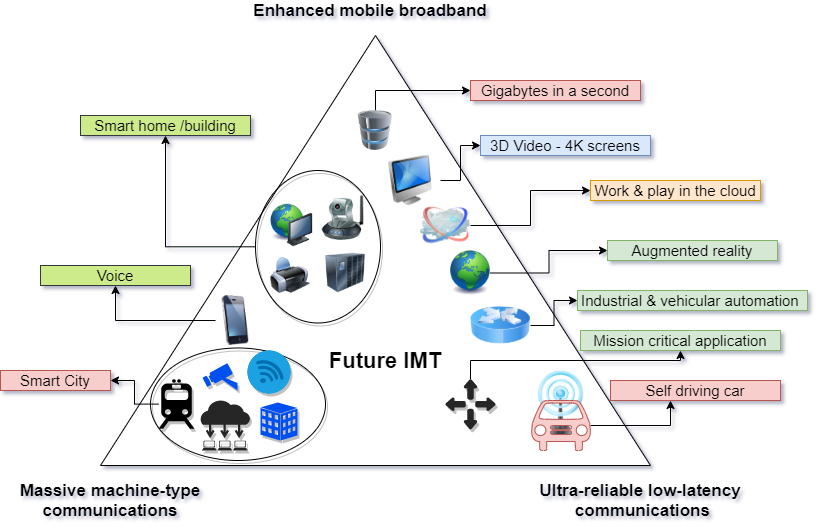
\includegraphics[scale=0.40]{images/IMT_2020_Use-cases.png}
\caption{IMT 2020 Use cases \cite{rancy2016imt}}
\label{fig:IMT_2020_Use-cases}
\end{figure}

In order to reach the topic's goal, we need to dive into the details of 5G Network Architecture; That is, where we have 
Service-based architecture (SBA) outlines the network function (e.g., AMF), and Reference point architecture proves how the Network function services are interacting with the Network function (NF)\cite{5G_Tech_Spec_Group_Ser2018study}.
This paper summarily describes the favorable deployment scenario for an integrated 5G and TSN system in Industry 4.0 field. Additionally, the Integration concepts will clarify the transparent and non-transparent approaches (represented in Tunneling, gateways, and proxies) \cite{ Eri_Gar_Theo_Oper_TSN2017study} \cite{Neumann2018}. \hfill \break
Last but not least, the following chapters will explain the details, including establishing a Protocol Data Unit (PDU) session between ingress TSN Translator (TT) and egress TT over Ethernet, and the required functions that need to be supported by the Open Source 5GC.




\begin{figure}

\centering
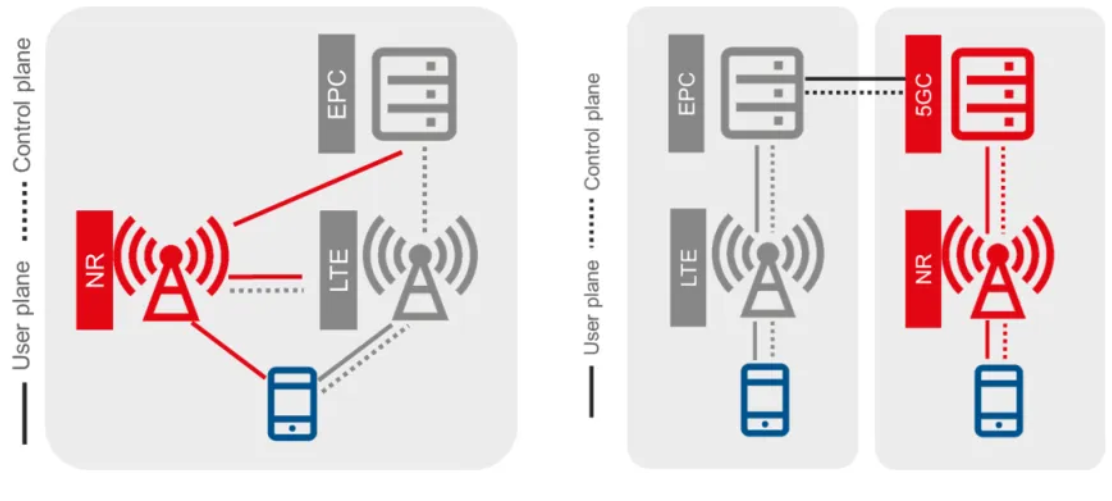
\includegraphics[scale=0.50]{images/SA_and_NSA_Architecture.png}
\caption{SA and NSA  Architecture\cite{Gsma_5G_implguid_study}.}
\label{fig:SA_and_NSA_Architecture}
\end{figure}




 %\hfill \break
 
\section{\textbf{Problem Statement}}\label{Problems} 

\subsection{Reliability and Low Latency}\label{Reliable and Low Latency}

Enhanced mobile broadband (eMBB) term is already in handling in 4G Networks. However,  For 5G, two fundamental classifications have been determined: massive machine-type communication (mMTC) to support an unlimited amount of associated nodes in industrial and consumer fields, and ultra-reliable low-latency communication (uRLLC) for critical communication and correlated control systems \cite{Ginthor2019}.
Figure \textbf{\ref{fig:5G_URLLC_TSN}} depicts the uRLLC features\cite{Ericsson2019}.


The abilities uRLLC empowers 5G to achieve the essential requests of time-sensitive communication, reliability, latency and wireless deterministic. According to the ITU-R\cite{series2017minimum}, Studies and research in 5G networks domain showed that End-to-End reliability is near to 99,999\% and latency of 1 ms of Data packets. However, the data rates higher to many Gb/s, processing entrance for up to a million devices per square kilometer.
5G Networks supports ultra-reliability for control and data channels by providing different techniques, such as encouraging multiple carriers and packet duplication over independent radio links, multi-antenna transmission.

Time-sensitive networking is a collection of Ethernet standards
currently developed by the IEEE 802.1 working group\cite{TSN2019_study}. TSN is an enabler of Industry 4.0 by providing flexible data access and full connectivity for a smart factory. The following reasons support this perspective, but we address them by mentioning and not limiting them. TSN empowers Industrial Automation by performing deterministic communication over Ethernet for real-time applications. By accomplishing scheduled traffic and synchronization, i.e., TSN grants guaranteed latency limitations \cite{Ginthor2019}.
On the other side, in a hybrid network, TSN supports many applications with various QoS requirements, e.g., closed-loop control, to grant the best-effort traffic over an individual standard Ethernet infrastructure\cite{Ericsson2019}. Figure \textbf{\ref{fig:Time-Sensitive_Networking(TSN)Profiles}} draws Time-Sensitive Networking (TSN) features (Selection and Use of TSN tools).



\begin{figure}

\centering
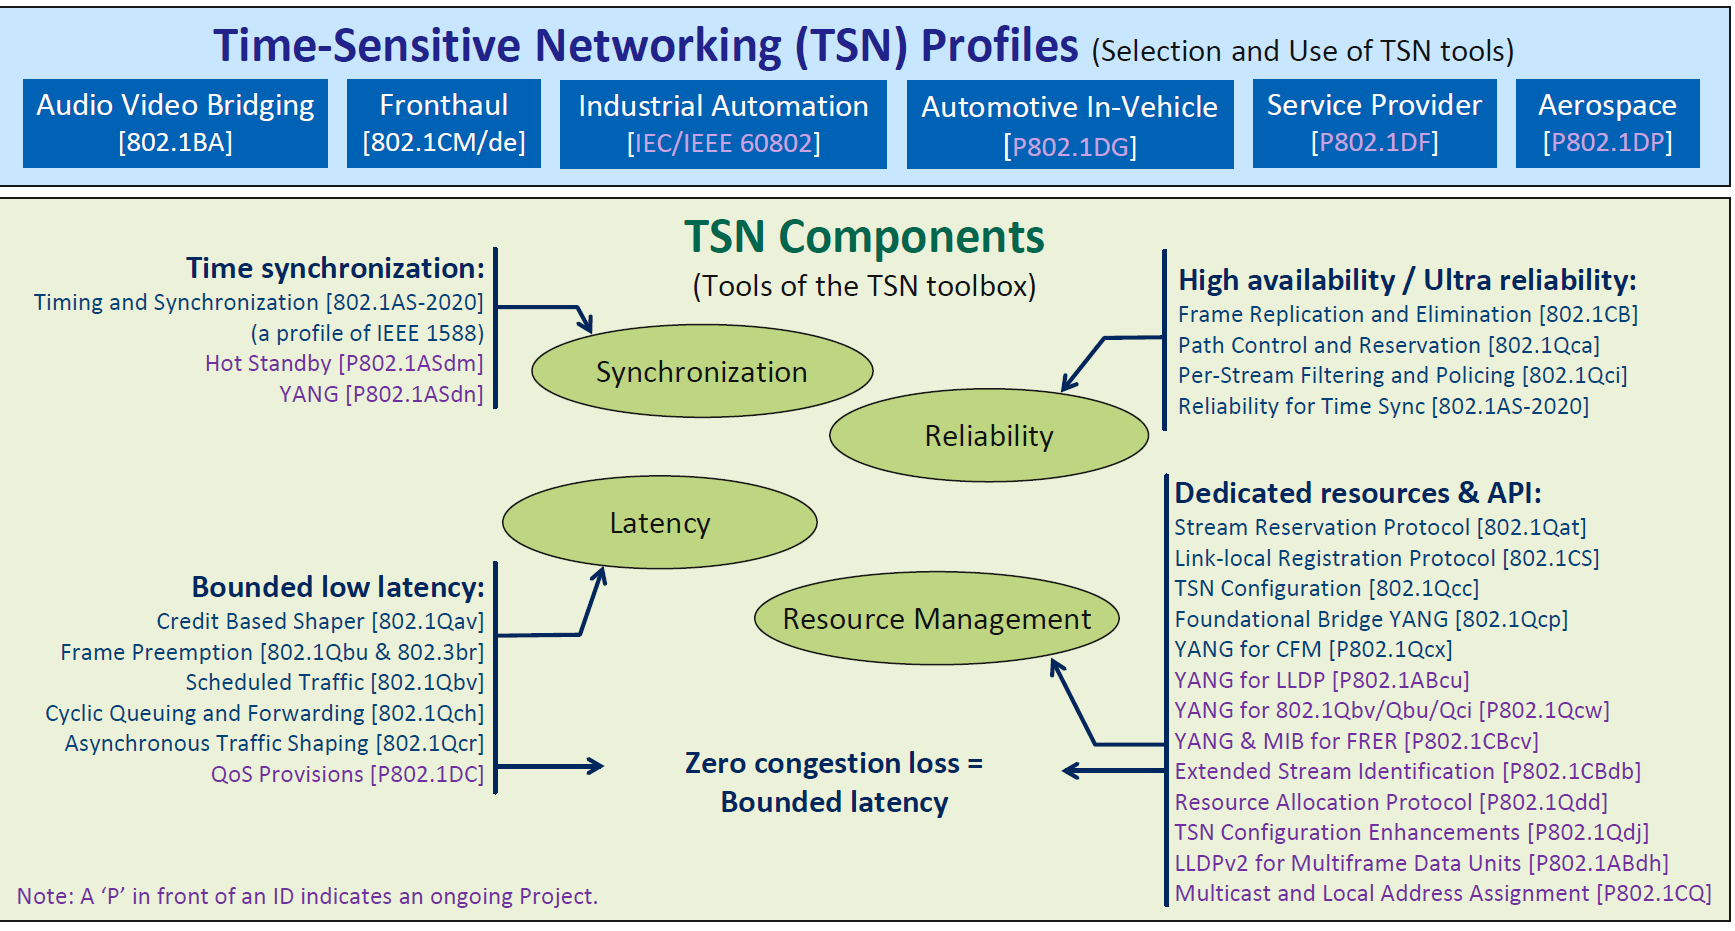
\includegraphics[scale=0.30]{images/Time-Sensitive_Networking(TSN)Profiles.png}
\caption{Time-Sensitive Networking (TSN) Profiles \cite{TSN2019_study}.}
\label{fig:Time-Sensitive_Networking(TSN)Profiles}
\end{figure}



\subsection{Real-Time (Wireless) Communications}\label{Real-Time (Wireless) Communications}
 
  %\hfill \break
  
 Wired networks have always played a primary role in industrial automation. However, the advantages and high efficiency of wireless communication demonstrated by performance indicators in smart manufacturing made it very attractive. Not only in the case of reducing energy consumption, expanding the range and increasing the bandwidth, but also in limiting packet collision. All this gives wireless networks flexibility and mobility. Nevertheless, the most significant factor for real-time systems is preventing collisions and thus ending data packets lost \cite{ring2012wireless}.
On the other hand, some applications like closed-loop control have a demand of periodic uRLLC, or uRLLC with a high refresh rate. This confirms that Synchronous and Hybrid Architecture for Real-Time (RT) Performance (SHARP) is the ideal solution. Which includes both required features uRLLC and Best-Effort traffic \cite{Seijo2019}. Therefore, the trend towards hybrid communication network systems was observed in the past and will continue into the future.
To address Real-Time (Wireless) Communications problems in industrial networks, previous mobile network generations and 5G cellular radio systems include Time synchronization as a fundamental element of their operation. Besides, the wireless network parts themselves are also time-synchronized, e.g., during the precision time protocol telecom profile \cite{ITU_TG82751_study}. All those features make it a strong candidate for time-critical systems. Figure\textbf{\ref{fig:5G_URLLC_TSN}} illustrates uRLLC features. There is a close relation between reliability and time synchronization, i.e., the draw reviews that 5G uses time synchronization for its operations, the multiple antennas, and radio channels that afford reliability\cite{Ericsson2019}. 5G also offers promising ideas and methods for managing low latency and resources, which can be combined to provide superior reliability and low latency.
What arouses curiosity; the 5G system (5GS) also contributes solutions in the core network (CN) for Ethernet networking and URLLC. The 5G CN offers native Ethernet protocol data unit (PDU) sessions. 5G assists in establishing unnecessary user plane paths through the 5GS, including RAN, the CN, and the carrier network. 5GS also allows for a redundant user plane separately between CN and RAN nodes and between the UE and the RAN nodes  \cite{Mannweiler2020}.



%%context

% ------------------------------------------------------------------------------
% (2) Why is it interesting and important? Why is it hard? (e.g., why do
% naive approaches fail?) Narrow down: what is problem you specifically
% consider? Describe the problem addressed in this paper.
% ------------------------------------------------------------------------------
%%\sidenote{importance}

% ------------------------------------------------------------------------------
% (3) Survey past work relevant to this paper. Why hasn't it been solved
% before (related work)? Or, what's wrong with previous proposed solutions? How
% does mine differ?
% ------------------------------------------------------------------------------
%%\sidenote{related work}
%%\todotext{One paragraph: Survey past work relevant to this paper. Why hasn't it been solved before (related work)? Or, what's wrong with previous proposed solutions? How does mine differ?}%%work

% ------------------------------------------------------------------------------
% (4) Define the own approach.
% ------------------------------------------------------------------------------
%%\sidenote{own approach}
%%\todotext{One paragraph: What is the own approach.}%%approach

% ------------------------------------------------------------------------------
% (5) What are the key components of my approach and results? Also include any
% specific limitations. It's the most crucial paragraph, tell
% your elevator pitch: How is it different/better/relates to other work?
% Help the reviewer to get the scientific surplus value between all
% the motivation and basics.
% ------------------------------------------------------------------------------
%%\sidenote{contribution}
%%\todotext{One paragraph: What is the surplus value of this paper.}%%result

% ------------------------------------------------------------------------------
% (6) How have we validated our results?
% ------------------------------------------------------------------------------
%%\sidenote{evaluation}
%%\todotext{One paragraph: How have we validated our results?}%%evaluation

% ------------------------------------------------------------------------------
% (7) How could this work be extended?
% ------------------------------------------------------------------------------
%%\sidenote{outlook}
%%\todotext{One paragraph: ow could this work be extended?}%%outlook

% ------------------------------------------------------------------------------
% (8) ``The remainder of this paper is structured as follows...''. The last
% section must give an overview of the paper.
% ------------------------------------------------------------------------------
% ------------------------------------------------------------------------------
 
 
 
 
    \section{\textbf{Existing Work }}\label{sec:relatedwork}
To place the paper's contribution in context and identify the gap the work is intended to fill, a short literature survey will provide.
We will touch on a brief overview of industrial automation's rival approaches, from Fieldbus to TSN, TSN over 5G in 3GPP Rel.15 and beyond. There were complete solutions and methods to connect field controllers, sensors, and actuators, which Fieldbus technology has granted\cite{thomesse2005fieldbus}. Those make it flexible regarding the architecture and give it the ability to support particular Qos for different applications. Nevertheless, Fieldbus Foundation, a not-for-profit organization, designed standards that increase operability, safety, therefore lowering cost when employing Fieldbus technology. Hence Fieldbus Foundation could guarantee the tested devices to ensure that they meet Fieldbus Foundation specifications and identified with \textsurd FF  for interoperability assurance. Consequently, Fieldbus technology was the ideal solution, and it took over at the A level in industrial automation from 1970 until November 2012, when the TSN Task Force was formed\cite{shoshani2010industrial}.
Time-sensitive networking (TSN) is a collection of standards under development by the IEEE 802.1 \cite{TSN2019_study}.The race was frantic among engineers and researchers working in industrial automation to make wired networks meet the need for time-critical systems. The reason for this was the inefficiency of the original IEEE 802.3 Ethernet standard. Besides, protocols based on Ethernet, like TCP, UDP, and IP, typically do not recognize real-time requirements.
The race was frantic among engineers and researchers working in industrial automation to make wired networks meet the need for time-critical systems. The reason for this was the inefficiency of the original IEEE 802.3 Ethernet standard. Besides, protocols based on Ethernet, like TCP, UDP, and IP, typically do not recognize real-time requirements. Therefore, the Open Systems Interconnection model (OSI model) modification rises to the highest level to match the conditions of the real-time application, which gives a strong impetus to improve the Industrial Ethernet schemes abilities. i.e.,
To overcome obstacles to standard Ethernet and protocol compatibility TCP/IP or UDP/IP with real-time systems requirements\cite{danielis2014survey}. Nevertheless, Ethernet's progress constant over the decades has seen its way into protocols such as Profinet, PowerLink, EtherCAT, and EtherNet/IP \cite{thomesse2005fieldbus}.
  


  \begin{figure}

\centering
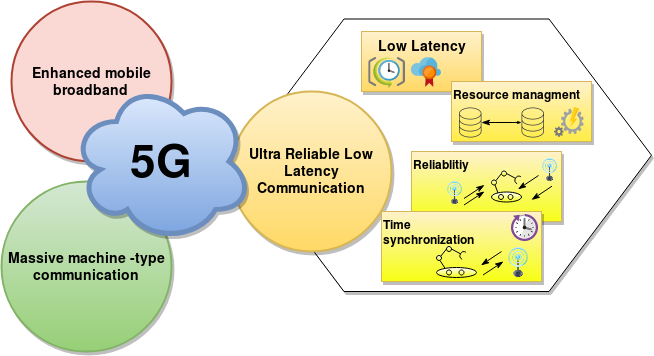
\includegraphics[scale=0.45]{images/5g-tsn-etr-figure01.png}
\caption{5G URLLC overview of TSN components \cite{Ericsson2019}}
\label{fig:5G_URLLC_TSN}
\end{figure}
 
  

\begin{figure}

\centering
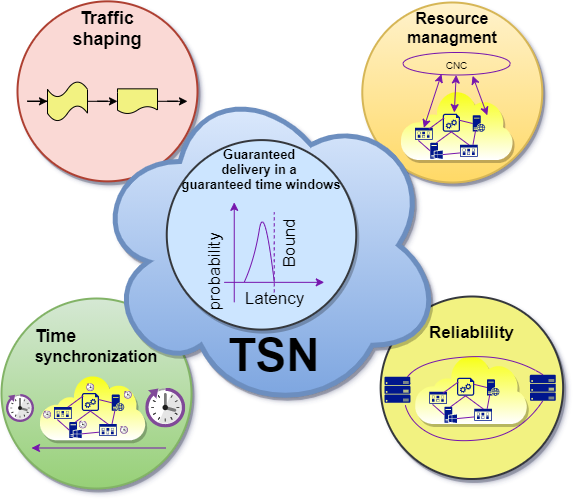
\includegraphics[scale=0.45]{images/TSN toolbox.png}
\caption{Valuable tools within the TSN toolbox that enable deployments in industrial automation \cite{embeddedcomputing2020}.}
\label{fig:TSN_toolbox}
\end{figure}
 

% -------------------------------------------------------------------------------
% The literature survey is a broad and shallow account of the field, which helps
% to place the contribution of the paper in context. It is part of the motivation
% of the paper, because it helps to identify the gap that this work is trying to
% fill, and explain why it is important to fill this gap. Rather than a list of
% disconnected accounts of other people's work, you should try to organise it
% into a story: What are the rival approaches? What are the drawbacks of each?
% How has !the battle between different approaches progressed? What are the major
% outstanding problems? (This is where you come in.)
% -------------------------------------------------------------------------------
\sidenote{intro}
As a review from the above, TSN standards are essentially for IEEE Std 802.3 Ethernet, which indicates they employ all the advantages of standard Ethernet, such as universality, flexibility, and economic operation price.
Various worthy tools are included in those standards like reliability, time synchronization, traffic shaping, resource management, as shown in figure
\textbf{\ref{fig:TSN_toolbox}}
TSN characteristics are developed upon the base IEEE 802.1 bridging standards, making them vital to be carried in industrial automation.


3GPP also provided the conditions for high data rates and traffic densities in 3GPP TS 22.261\cite{5G_Ser_req_nex_gen2018study}; in this 50Mbps is the essential requirement of eMBB service for down link (DL). Up Link (UL) and DL requirement for high data rates and traffic densities can be seen in the \textbf{table}
\textbf{\ref{table:Performance_requirements_highdatarates_traffic_densities}}. 
 



  
%\todoshort{This survey focuses on \ac{WATER} and \ac{Greedy Computing}\ldots\ac{Greedy Computing}}.

%\sidenote{gap 1}
%\todotext{related work 1}



\begin{table}[h!]
\centering
\begin{tabular}{|p{1.8 cm}| p{1.8 cm} |p{1.8 cm}| p{2 cm}| p{2 cm}| p{2 cm}|} 


 \hline
 \cellcolor[HTML]{23a5e2} \color[HTML]{ffffff} \textbf{Scenario} &\cellcolor[HTML]{23a5e2} \color[HTML]{ffffff} \textbf{Experience data rate (DL)}  & \cellcolor[HTML]{23a5e2} \color[HTML]{ffffff} \textbf{Experience data rate (UL)} &\cellcolor[HTML]{23a5e2}\color[HTML]{ffffff} \textbf{Area Traffic Capacity (DL)}   &\cellcolor[HTML]{23a5e2} \color[HTML]{ffffff} \textbf{Area Traffic Capacity (UL)}    & \cellcolor[HTML]{23a5e2}\cellcolor[HTML]{23a5e2} \color[HTML]{ffffff}\textbf{Overall user density }  \\ 
 \hline
 Urban & 50 Mbps &   25 Mbps &  100 \break   Gbps/km2 &     50 \break $Gbps/km^2$  &   $10000/km^2$   \\ 
  \hline
 Rural &     50  Mbps &  25   Mbps &   1 \break   $Gbps/km^2$  &  500 \break  $Gbps/km^2$  & $100/km^2$  \\
  \hline
 Indoor hotspot &    1 Gbps &    500 Mbps &  15  \break   $Tbps/km^2$  &    2 \break $Tbps/km^2$  &   $250000/km^2$  \\
  \hline
 Dense urban &   300 Mbps &  50 Mbps &   750 \break  $Gbps/km^2$  &  125 \break   $Gbps/km^2$  &  $25000/km^2$  \\
  \hline
High- speed vehicle &    50 Mbps &   25 Mbps &    100  \break  $Gbps/km^2$  &   50  \break $Gbps/km^2$  &   $4000/km^2$  \\ [1ex] 
 \hline
\end{tabular}
\caption{Performance requirements for high data rates and traffic densities\cite{5G_Ser_req_nex_gen2018study}.}
\label{table:Performance_requirements_highdatarates_traffic_densities}
\end{table}



\begin{figure}
\centering
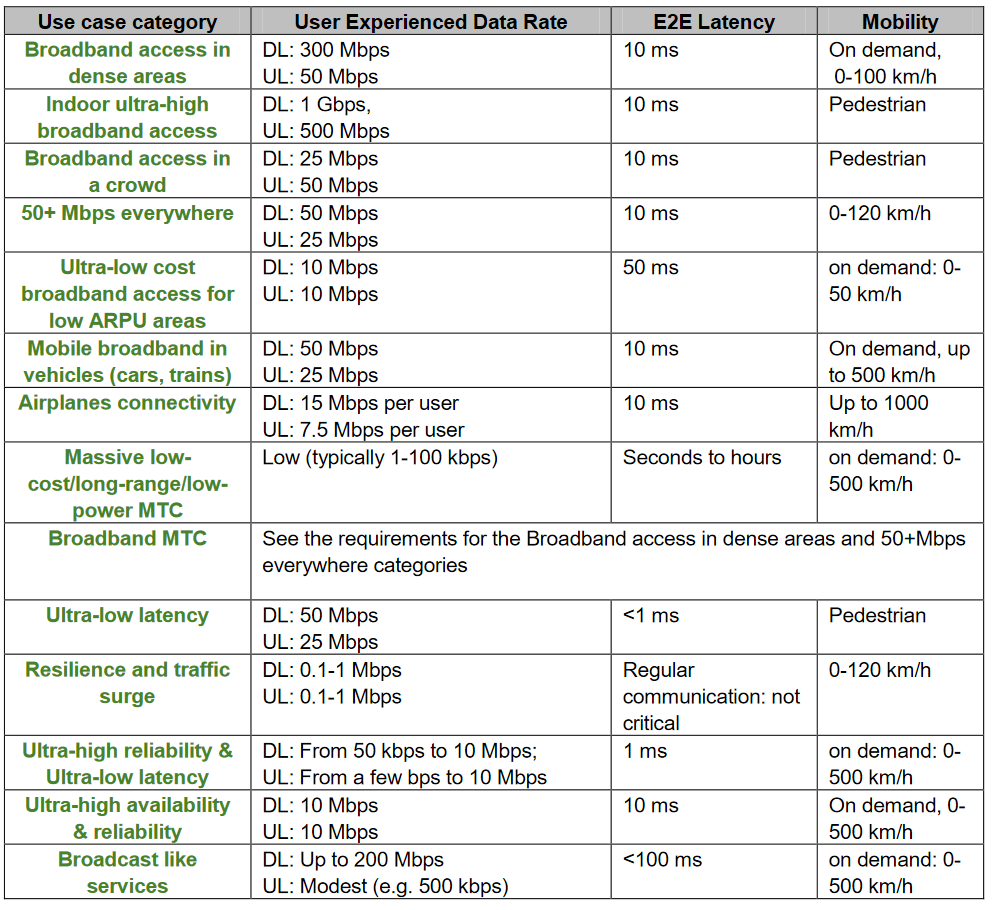
\includegraphics[scale=0.58]{images/User Experience Requirements.png}
\caption{User Experience Requirements\cite{alliance20155g}.}
\label{fig:User_Experience_Requirements}
\end{figure}



\subsection{5G Network Architecture}
3GPP determined the specification of the 5G architecture. 3GPP defined the 5G architecture
in two methods, first as a service-based and the second reference point architecture, which shows the intercommunication between network functions \cite{5G_Tech_Spec_Group_Ser2018study}.
\begin{itemize}
    \item Service-based architecture (SBA) describes the network function (e.g., AMF) of the control plane and also defines how it can authorize other network functions to access the services of other network functions. You can see the SBA in figure \textbf{\ref{fig:5G_SBA}
    \item Reference point architecture explains how the NF services are interacting with the Network function. All of these interactions represented by a point-to-point reference (e.g., N5) between two network functions (e.g., UDM and NRF).  As it shown in figure} \textbf{\ref{fig:5G_Reference_Point_Architecture}}
\end{itemize}


\begin{figure}

\centering
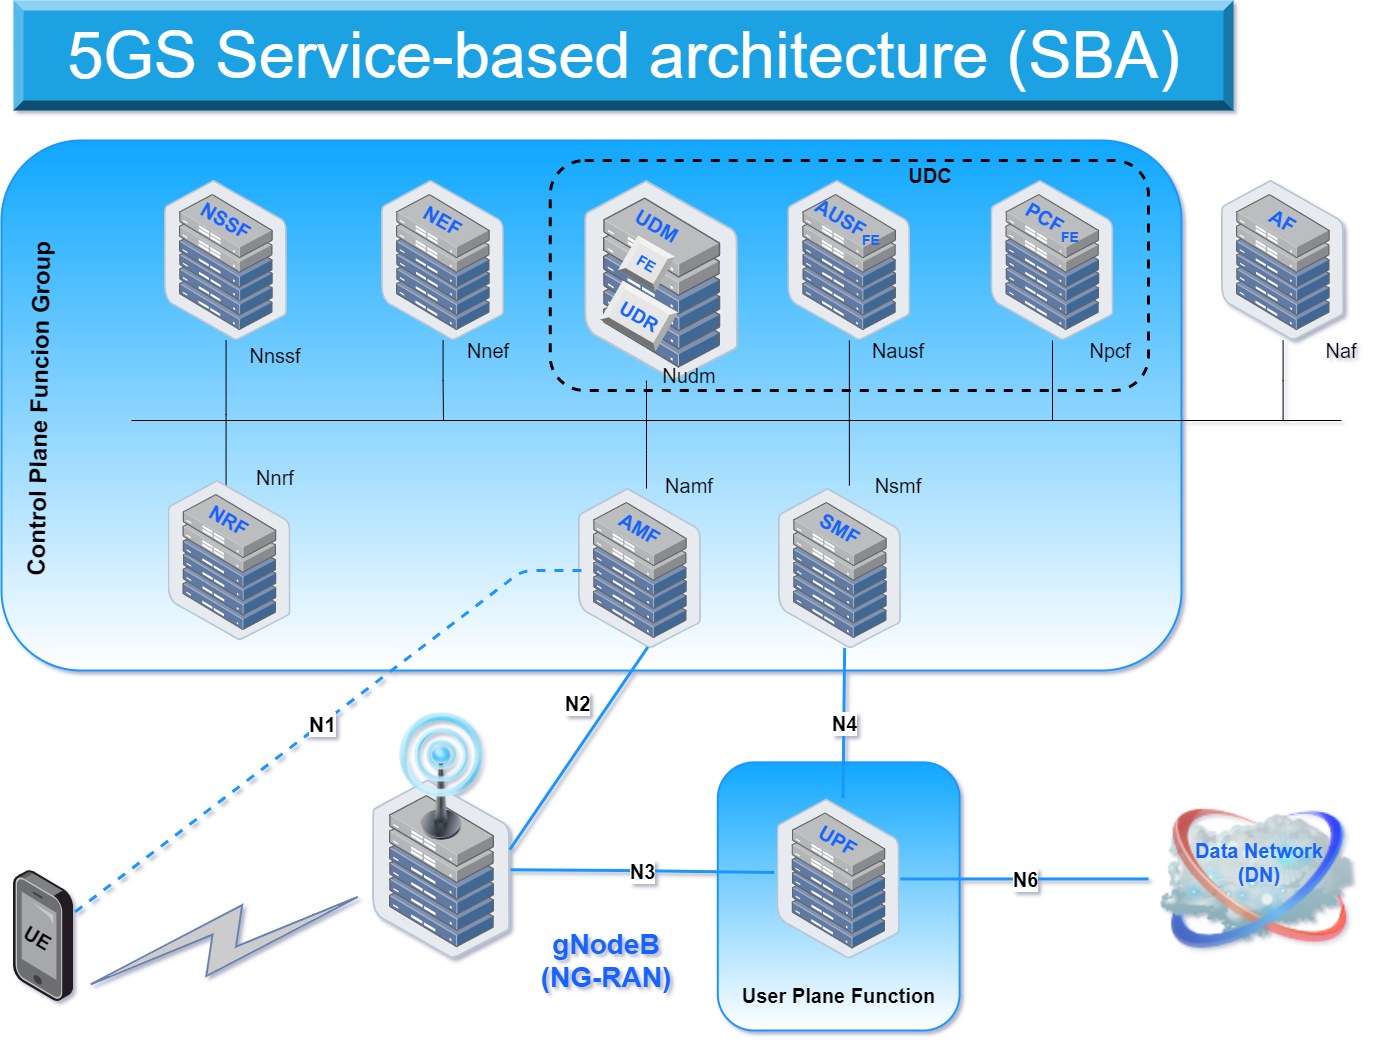
\includegraphics[scale=0.25]{images/5G_SBA.png}
\caption{5GS Service-based architecture (SBA)\cite{5G_Sys_arch_5Gsystem2018study}.}
\label{fig:5G_SBA}
\end{figure}
 
  
\begin{figure}

\centering
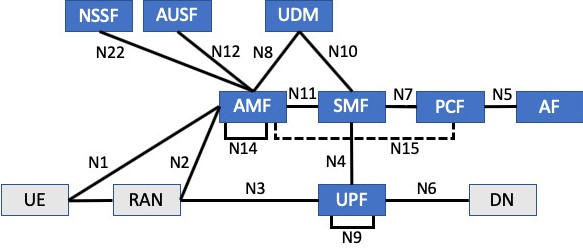
\includegraphics[scale=0.60]{images/5G_Reference_Point_Architecture.png} 
\caption{5G Reference Point Architecture}
\label{fig:5G_Reference_Point_Architecture}
\end{figure}

All essential elements of our research are discussed in the 3GPP release 15 specifications when the 5G service-based architecture (SBA) was reviewed. The fundamental technological components in the 5G core network are the separation of control plane and user plane, service-based interface (SBI), modularization, and network function virtualization. SBA Architecture provides a single API calling interface.  All the network functions (NF) are interconnected via an interface for calling the other NF. 
After Authorization, the network functions (NFs) able to access the other NF using SBI. Network function virtualization (NFV) empowers the network function to be virtualized and deployed on any cloud environment. The support of virtualization in the 5G, the limits between traditional Evolved Packet Core (EPC) network components (MME, SGW, and PGW) will come to exit \cite{5G_Tech_Spec_Group_Ser2018study}.

In 5G Service-Based architecture, Many advantages noticed; independent logical network, sharing the infrastructure either wholly or partly, and being deployed on different infrastructure. I.e., 5GC  Supports network slicing. Furthermore, SBA interfaces are beneficial; 5GC promotes working with 3rd parties and can customize network slice capabilities via AF\cite{5G_Tech_Spec_Group_Ser2018study}.
Another important feature; 5G architecture empowers us to take full advantage of the most advanced virtualization and software technologies. The SBA architecture provides a foreseen performance and flexibility for the network. The following are the 5GC network functions\cite{5G_Sys_arch_5Gsystem2018study}:
\begin{itemize}
    \item AMF: Access and Mobility Management Function - PCF: Policy Control Function.
    \item SMF: Session Management Function - UPF: User Plane Function.
    \item NRF: Network Repository Function - AF: Application Function
    \item NEF: Network Exposure Function - UDM: User Data Management.
    \item AUSF: Authentication Server Function - NSSF: Network Slice Selection Function.
    \item SBI: Service Based Interfaces (Namf, Nsmf, Nudm, Nnrf, Nnssf, Nausf, Nnef, Nsmsf, Nudr, Npcf)
 
\end{itemize}



\textbf{Table}
\textbf{\ref{table: 5G_interfaces_and_the_functional_Description}}  indicates 5G Interfaces and Functional Description of them.
\hfill \break
Another significant technical concept is Network Slicing, clearly “5G slice”, which strengthens the communication service of a particular connection model with a particular method of handling the User-Plane and Control-Plane for this service. To this purpose, a 5G slice is composed of 5G network functions (NF) and precise RAT settings combined together for the exact use case or business model.
figure
\textbf{\ref{fig:Network_Slicing_for_different_use-cases}} represents an instance of multiple 5G slices concurrently served on the same infrastructure\cite{alliance20155g}. 
 
 \begin{table}[h!]
\centering
\begin{tabular}{|p{2.3cm}| p{8.5 cm} |} 

 \hline
 \cellcolor[HTML]{23a5e2} \color[HTML]{ffffff} \textbf{5G interfaces} &\cellcolor[HTML]{23a5e2} \color[HTML]{ffffff} \textbf{Functional Description}    \\ 
 \hline
N1 & Between UE and AMF (Access and Mobility Management Function)  \\ 
  \hline
N2 & Between RAN (Radio Access Network) or gNB (i.e. 5G base station) and AMF  \\ 
  \hline
N3 & Between RAN or gNB (i.e. 5G base station) and UPF (User Plane Function) \\ 
  \hline
N4 & Between SMF (Session Management Function) and UPF
  \\ 
 \hline
  N5 & Between PCF (Policy Control Function) and AF (Application Function).
  \\ 
  \hline
N6 & Between UPF and DN (Data Network)
  \\ 
  \hline
N7 & NG7 is reference point between SMF and PCF 
  \\ 
  \hline
N8 & Between Unified Data Management (UDM) and AMF  \\ 
  \hline
N9 &  Between two core UPFs \\ 
\hline
  N10 &  Reference point between UDM and SMF\\ 
  \hline
N11 & Between SMF and SMF  \\ 
  \hline
N12 & Between AMF and AUSF (Authentication Server Function)    \\ 
  \hline
N13 & Between UDM and AUSF  \\ 
  \hline
N14 & Between two AMFs  \\ 
\hline
  N15 & Between PCF and AMF (in Nonroaming scenario)  \\ 
  \hline
\end{tabular}
\caption{Shows the 5G Interfaces and Functional Description.}
\label{table: 5G_interfaces_and_the_functional_Description}
\end{table}

 
 
 
 
 
 
 
 
 
 
 


\begin{figure}

\centering
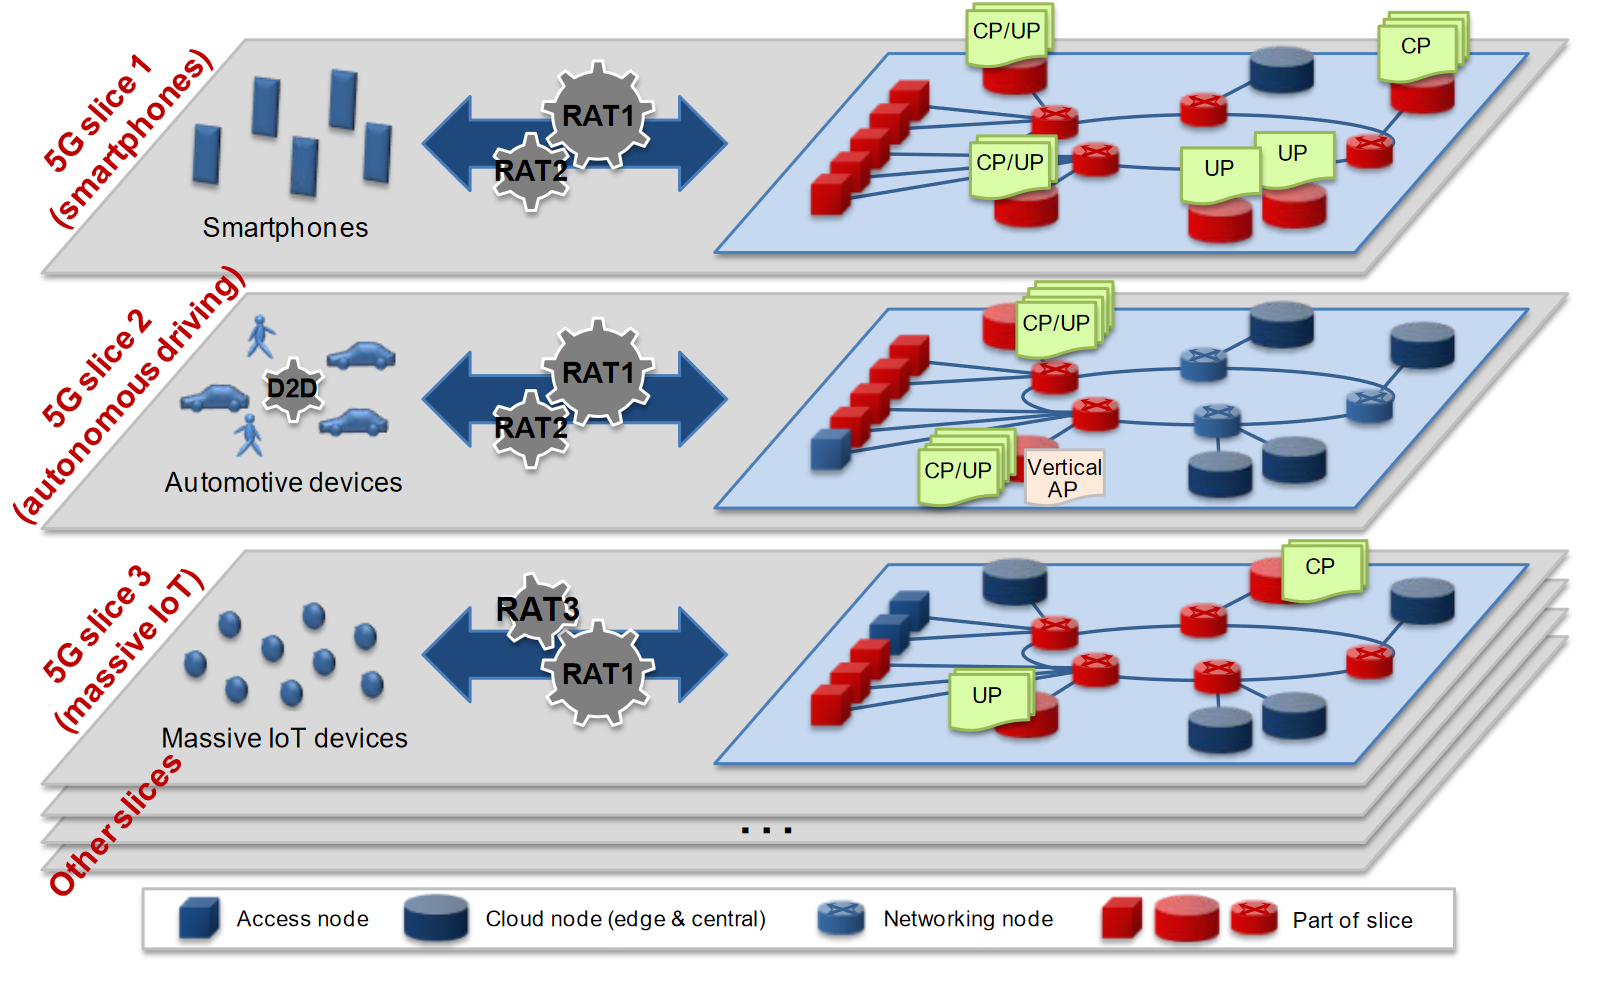
\includegraphics[scale=0.33]{images/Network Slicing for different use-cases.png}
\caption{Network Slicing for different use-cases \cite{alliance20155g}.}
\label{fig:Network_Slicing_for_different_use-cases}
\end{figure}


\subsection{5GC-TSN Integration Scenarios}
The Integration of the 5G core network and TSN has many possibilities. This Thesis will handle three scenarios of them. Every scenario has its unique advantages to award them to particular user applications\cite{5gacia2021_study}. 
 
\begin{itemize}
    \item Scenario 1:
     Within the first scenario, we have the production sectors for the production area. The connection between those isles is using Industrial Ethernet technology \cite{5gacia2021_study}.
Consequently, all communication endpoints give network interfaces according to a similar model. In this scenario, 5GS supports the data interchange amongst the isles, which becomes a demand in Industry 4.0 and digitization \cite{Seijo2019}. 
In this instance, figure
\textbf{\ref{fig:Scenario_1-Connected_homogeneous_islands}}
 shows that 5GC networks are not affected by this scenario, while the focus is restricted to the Radio Access Network (RAN) and the backhaul of the 5GS figure}
\textbf{\ref{fig:The_role_5GS_bridgesindustrial_automation}(A)}.


\begin{figure}

\centering
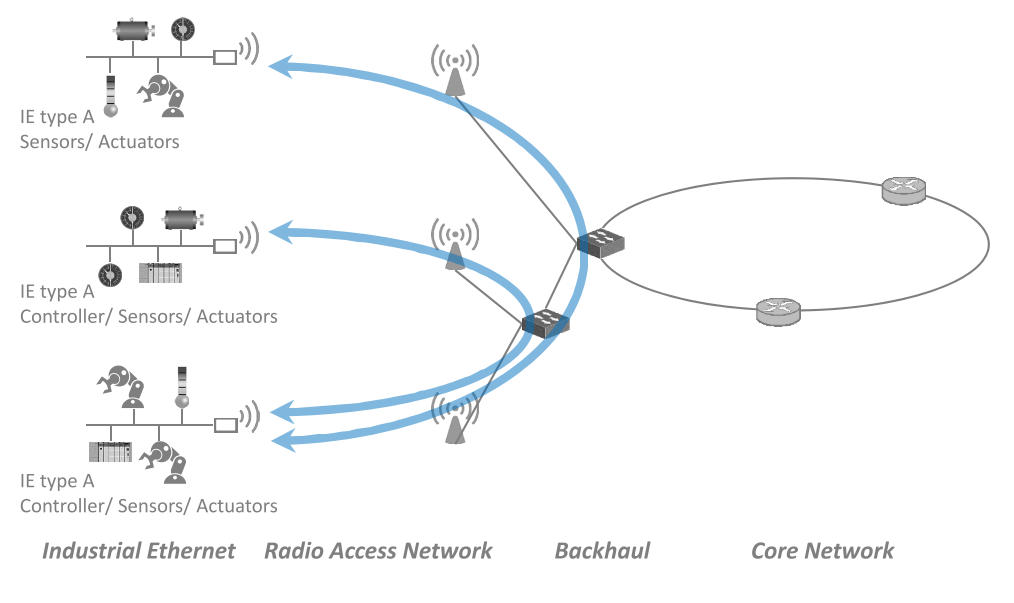
\includegraphics[scale=0.50]{images/Scenario 1- Connected homogeneous islands.png}
\caption{Scenario 1: Connected homogeneous isles \cite{Neumann2018}.}
\label{fig:Scenario_1-Connected_homogeneous_islands}
\end{figure}


\item Scenario 2:
      

This scenario is an ideal decision for utilizing cloud-based control \cite{givehchi2014control}. The motivation of that is working mechanism and structure. I.e., as a main noticed difference between the first and second scenario, the controller's physical object is moved from an allocated machine at the production line to a virtualized entity in the 5G network\cite{5gacia2021_study}. The complete 5GS is covered in this scenario; since the virtualized controller is connected to the core network. In figure \textbf{\ref{fig:Scenario_2_Virtualized_controller}}, we figure out that, Qos is required at a high level because the entire 5G layout is considered in the control loop. The virtualized controller performs a standard Ethernet IP-based connection\cite{5gacia2021_study}. Conversely, two access methods: Industrial Ethernet or native 5G radio, probably are donated by the actuators or sensors at the production line
figure
\textbf{\ref{fig:The_role_5GS_bridgesindustrial_automation}(B)}.

\begin{figure}

\centering
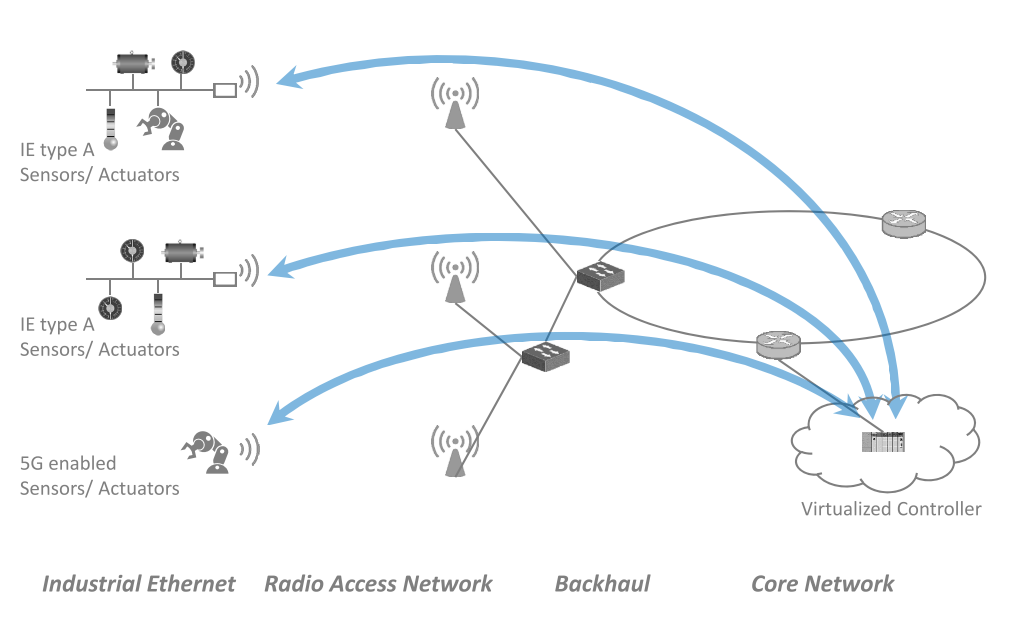
\includegraphics[scale=0.50]{images/Scenario 2- Virtualized controller.png}
\caption{Scenario 2: Virtualized controller \cite{Neumann2018}.}
\label{fig:Scenario_2_Virtualized_controller}
\end{figure}
    
    
    \item Scenario 3:
 A surprise that snatched the spotlight between the three scenarios is scenario 3 shown in figure
\textbf{\ref{fig:The_role_5GS_bridgesindustrial_automation}(C)}. It is similar to the second scenario in terms of a  virtualized controller but is distinct from its design, including a remote production entity connected to 5GC Network \cite{5gacia2021_study}. Hence, its significant advantage demonstrates by supporting various types of communications technologies: 5G radio, standard Ethernet IP-based protocols,  and different Industrial Ethernet protocols.
Scenario 3 diagram illustrated in figure
\textbf{\ref{fig:Scenario_3_Versatility_with_virtualization_&_remote_site}}.



\begin{figure}

\centering
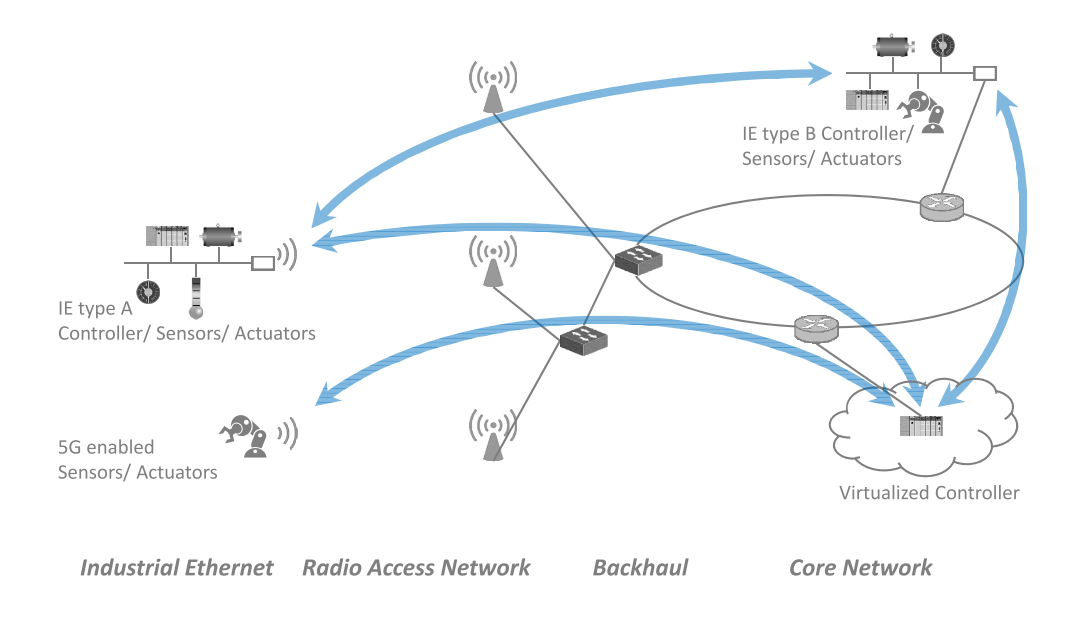
\includegraphics[scale=0.50]{images/Scenario 3- Versatility with virtualization and remote site.png} 
\caption{Scenario 3: Versatility with virtualization and remote site \cite{Neumann2018}.}
\label{fig:Scenario_3_Versatility_with_virtualization_&_remote_site}
\end{figure}


%end scenarios
\end{itemize}
The mentioned scenarios have the feasibility to apply through many use cases of 5GC-TSN integration, which takes its ways in Industrial automation \cite{3gpp2018study}.
Domains that could benefit from the first scenario include;
mobile robots, closed-loop control in process automation, connectivity for the factory floor, mobile control panels, or modular assembly areas. On the other hand, Scenario 2 concerns control-to-control communication, process monitoring, extensive sensor networks,  plant asset management. Last but not least, Scenario 3 is fit for inbound logistics or remote access and maintenance \cite{Neumann2018}.

In addition, Mobility indicates the system’s ability to support continuous service activity for movable users. Furthermore, the identified 5G use cases show that 5G networks will support an increasingly large spectrum of static users/devices to mobile users. 
Regardless of the massive support for 5G networks of a large number of mobile and fixed nodes, 5GS should support mobility-on-demand only. From low mobility or stationary devices like smart meters to very high mobility, like high-speed trains/airplanes \cite{alliance20155g}. In all cases, the conditional speed between the network edge and the user refers to the mobility needs. In other words,  The harmony of the user's activity must be guaranteed.  Use case specific mobility requirements are shown in figure
\textbf{\ref{fig:User_Experience_Requirements}}.




\begin{figure}

\centering
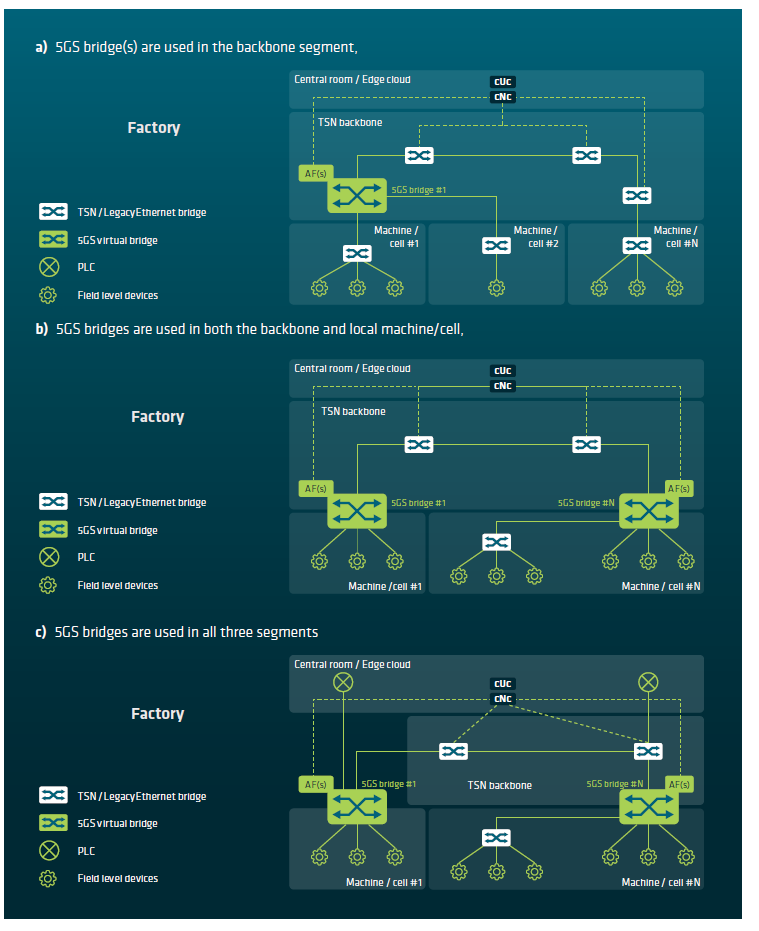
\includegraphics[scale=0.60]{images/The role of 5GS bridges in industrial automation.png} 
\caption{The role of 5GS bridges in industrial automation\cite{5gacia2021_study}.}
\label{fig:The_role_5GS_bridgesindustrial_automation}
\end{figure}


    \section{\textbf{Own approach }}\label{sec:main}
 
 
This part will identify TSN requirements over 5G testbed and the automatic setup of selected open-source 5G testbed.
 \subsection{The integration of 5G with TSN configuration approach}
 
The Thesis will deal with the use cases of integration 5G-TSN  in the Manufacturing Domains, where 5G technology does not has any action on  E2E protocols. I.e., This refers to the transparent methods of 5G-TSN integration\cite{Neumann2018}. On the contrary, the study will not discuss the non-transparent methods of 5G-TSN integration presented by Tunneling, gateways, and proxies. By reason of not being able to meet requirements of the combining of 5G and TSN.

 
Other related concepts are P802.1Qcc, and Stream Reservation Protocol (SRP) Enhancements and Performance Improvements \cite{TSN2019_study}. 802.1Qcc enables the coexistence between centralized configuration management and decentralized configuration, configurable SR (stream reservation) classes and streams, benefits heterogeneous configurations for legacy Audio Video Bridging (AVB) equipment \cite{kreifeldt2009avb}, support for Layer 3 streaming, fully centralized configuration, deterministic stream reservation convergence, and fully distributed configuration of the Stream Reservation Protocol (SRP)\cite{TSN2019_study}. TSN Configuration fully distributed model showed in figure \textbf{\ref{fig:TSN_Configuration_fullydistributed[802.1Qcc]}}.
\begin{itemize}
    \item Fully centralized configuration of IEEE 802.1Qcc: Regarding IEEE 802.1 sense, the system is classified into two characters of equipment: bridges and end stations (Talker or Listener) \cite{TSN2019_study}.
    The talker end station is the source or a machine that generates data, e.g.,  (sensors). The listener end station is the destination or a machine that receives and uses data, e.g., controller or monitoring device \cite{Eri_Gar_Theo_Oper_TSN2017study}. Stream: a unidirectional movement of data from a Talker to one or more further Listeners. As depicted in 
    figure \textbf{\ref{fig:802.1Qcc_Fully_Centralized_Configuration_Model}},  the technology consists of the following elements: Centralized User Configuration (CUC), Centralized Network Controller (CNC), and Bridges. The Bridge is a design , see figure \textbf{\ref{fig:Bridge_Architecture}}, that includes Media Access Control (MAC) Bridge or Virtual Local Area Network (VLAN) Bridge element functionality \cite{Mannweiler2020}. Time-synchronization is at a high level in this topology. I.e., The topology has a collection of time-aware bridges. On the other hand, end stations and these bridges are synchronized to a master clock in the system. Besides, the complete network is sensible of the global time—however, The interaction between the previously mentioned elements detailed in figure \textbf{\ref{fig:CUC-CNC_Interactions_for_Industrial_TSN_Domain_Configuration}}. In addition, (CNC) deals with network devices (bridges), while (CUC) deals with user devices (end stations). The CNC and CUC present the control plane (CP) rather than distributed protocols; i.e., the fully centralized configuration model attends a software-defined networking (SDN) approach. In opposition, distributed control protocols are utilized in the fully distributed model, where there is no CNC or CUC \cite{Ericsson2019}.


    \begin{figure}
    \centering
    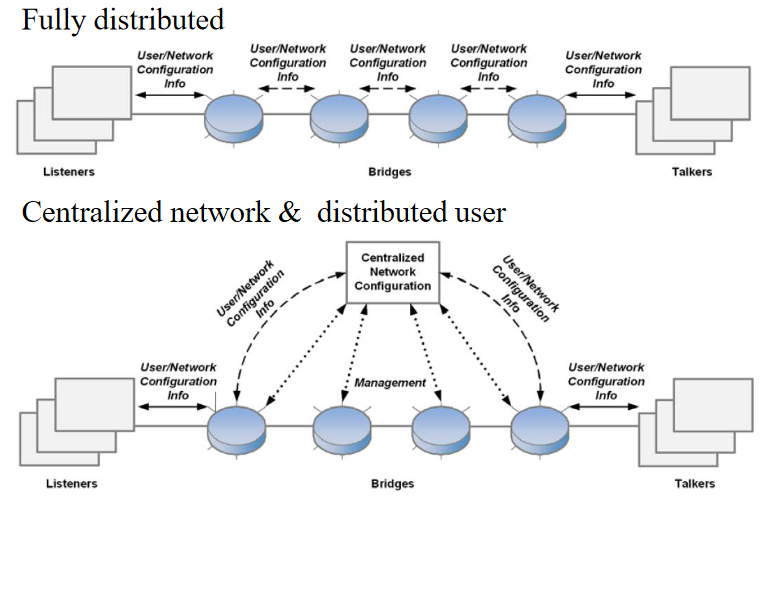
\includegraphics[scale=0.65]{images/TSN Configuration fully distributed [802.1Qcc].png} 
    \caption{TSN Configuration fully distributed [802.1Qcc] \cite{TSN2019_study}.}
    \label{fig:TSN_Configuration_fullydistributed[802.1Qcc]}
     \end{figure}
    
    
    \begin{figure}
    \centering
    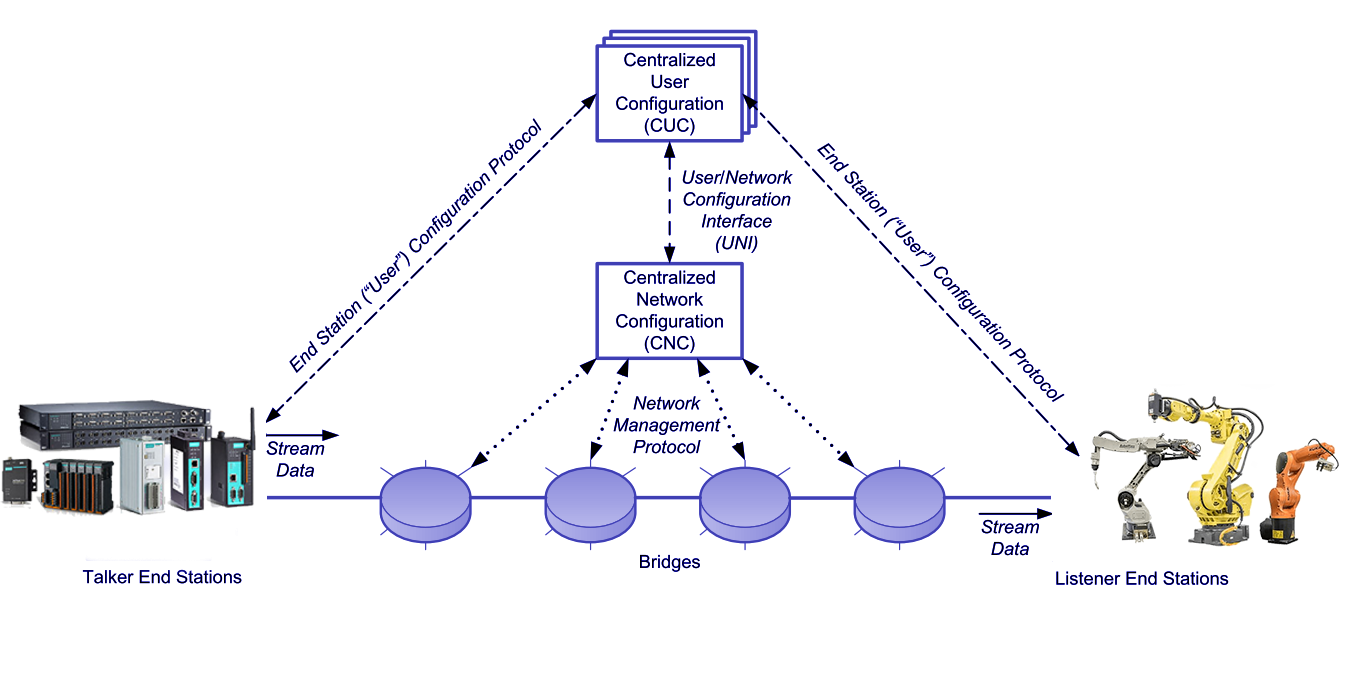
\includegraphics[scale=0.22]{images/802.1Qcc Fully Centralized Configuration Model.png} 
    \caption{802.1Qcc Fully Centralized Configuration Model \cite{Ginthor2019}}
    \label{fig:802.1Qcc_Fully_Centralized_Configuration_Model}
    \end{figure}


\begin{figure}
\centering
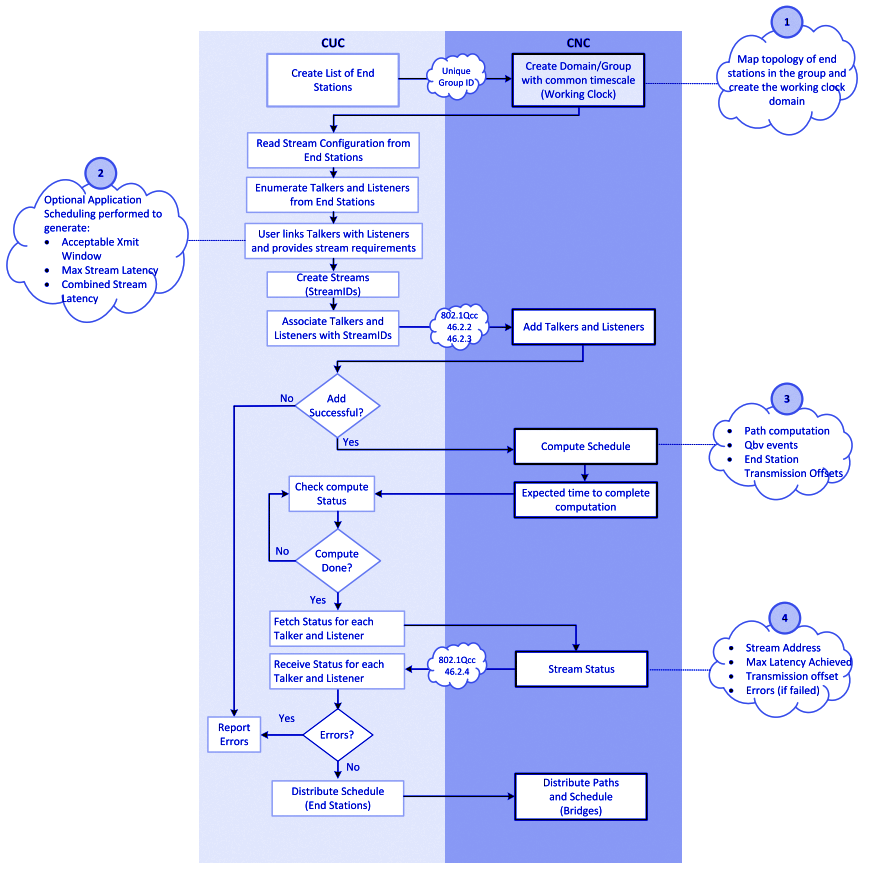
\includegraphics[scale=0.38]{images/CUC-CNC Interactions for Industrial TSN Domain Configuration.png} 
\caption{CUC-CNC Interactions for Industrial TSN Domain Configuration \cite{Eri_Gar_Theo_Oper_TSN2017study}.}
\label{fig:CUC-CNC_Interactions_for_Industrial_TSN_Domain_Configuration}
 \end{figure}


 
     \item 3GPP 5GS mobile network within TSN Transparent integration:
     In order to focus on the thesis goal, we perform a zoom in on a TSN bridge of the 802.1Qcc Fully Centralized Configuration Model, that illustrates in figure \textbf{\ref{fig:OS-5GC-Main}} considering TSN features that shown in figure
     \textbf{\ref{fig:TSN_toolbox}}. 
       Regarding 3GPP Release 16, two operative items are provided; TSN Translator (TT) and an adaptation interface (AIF). Both items represent the concept of the integration of 5G into TSN in industrial automation. I.e., TT and AIF encapsulate the 5G network as a virtual bridge in the TSN network. These two objects modify the TSN performances into identical movements in the 5G and vice versa.  Besides, within the TT functionality, the 3GPP 5GS empowers TSN bridge ingress and egress port additions. To characterize these two advantages, the TTs provide hold, and forward functionality for de-jittering \cite{Ericsson2019}. Link Layer Discovery Protocol (LLDP) and Precision Time Protocol (PTP) also play an essential operational purpose in promoting the integration \cite{Neumann2018}.
       We also note in the diagram showing the case of two TSN streams associated with two PDU sessions and two EU devices. Furthermore, other angles of the coexisting concept between 5G Network and TSN clarify by supporting 5GS the coherence process of bridges and joining an end station to a bridged network\cite{Ericsson2019}. The deployment contains only an actual UE among two PDU sessions utilizing duplicated connectivity in Radio Access Network (RAN).  Consequently, the entire 5G network will look like a TSN bridge.
     \end{itemize}


 \begin{figure}
\centering
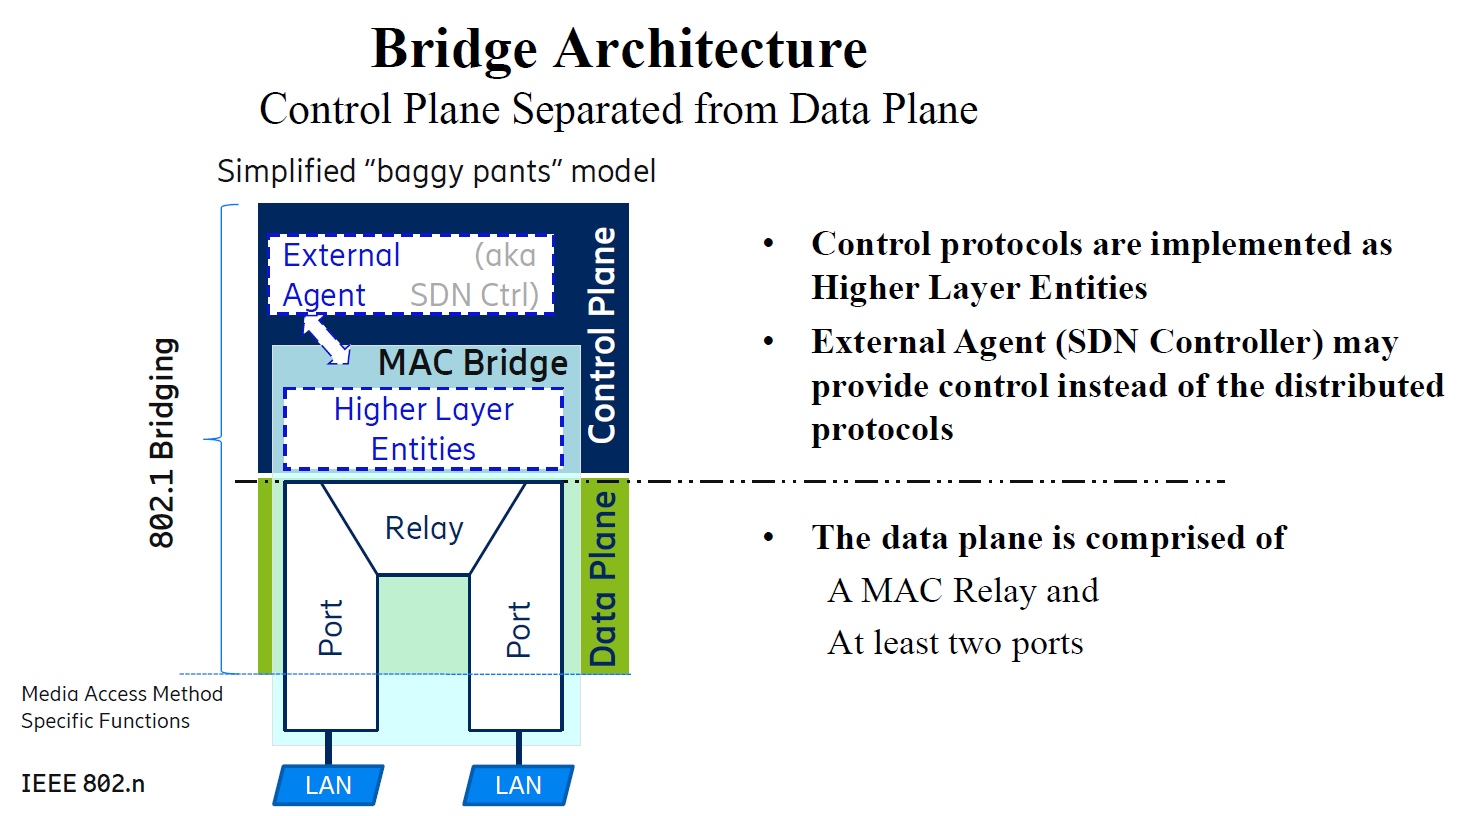
\includegraphics[scale=0.22]{images/Bridge Architecture.png} 
\caption{Bridge Architecture}
\label{fig:Bridge_Architecture}
 \end{figure}
 
 
 \begin{figure}
 
\centering
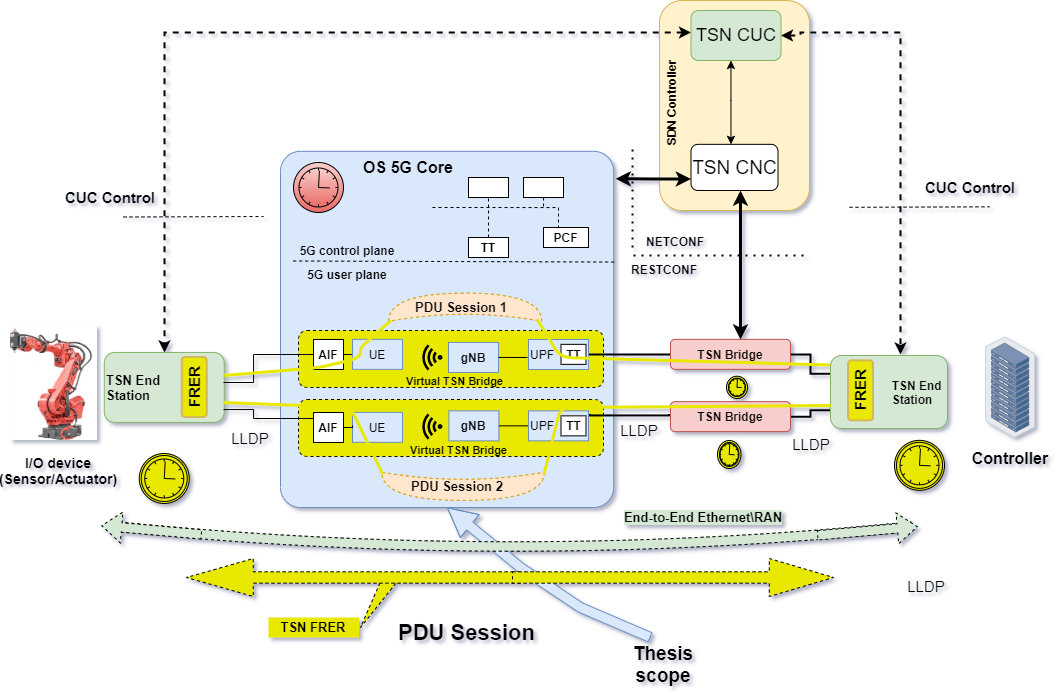
\includegraphics[scale=0.30]{images/OS-5GC-Main.png}
\caption{Open source 5G Core Testbed\cite{Ericsson2019}}
\label{fig:OS-5GC-Main}
  \end{figure}

 
 
 
 
We conclude from the above that The 5GC supports a Protocol Data Unit (PDU) Connectivity Service, i.e., a service that provides the exchange of PDUs between a UE and a data network identified by a Data Network Name (DNN) \cite{ROMMER2020111}. The PDU Connectivity Service is supported via PDU Sessions that are established upon request from the User Equipment (UE), between ingress TSN Translator (TT) and egress TT over Ethernet(not necessarily RAN between 5G base station GNodeB (gNB)  and User Equipment (UE)) as illustrated by figure \textbf{\ref{fig:OS-5GC-Main}}.
Typically, These PDUs can be IP, Ethernet, and Unstructured, besides DNN (Data Network Name) is employed to distinguish various destination networks outside these 5G networks. Figure \textbf{\ref{fig:Simplified_PDU_Session_Establishment_procedure}} represents a simplified PDU Session Establishment call flow, highlighting the key Network Functions included as well as the steps taken in the process \cite{ROMMER2020111}.

 
\begin{figure}
\centering
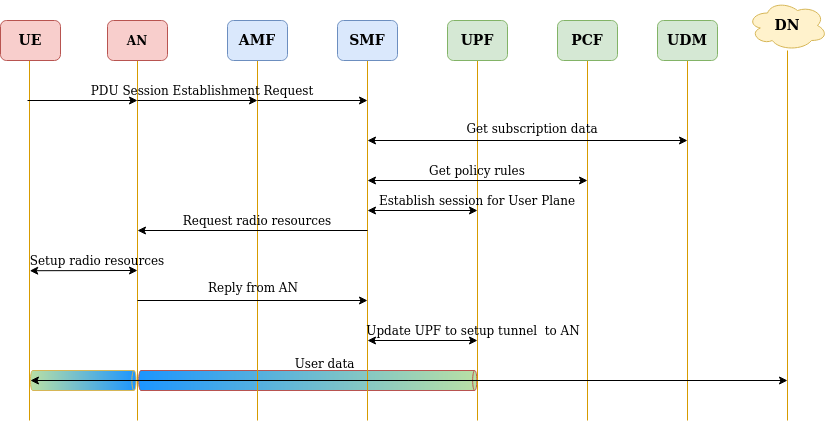
\includegraphics[scale=0.40]{images/Simplified_PDU_Session_Establishment_procedure.png} 
\caption{Simplified PDU Session Establishment procedure \cite{ROMMER2020111}}
\label{fig:Simplified_PDU_Session_Establishment_procedure}
 \end{figure}



 However, all universities and research institutes are closed due to the corona pandemic crisis these days. Nevertheless, Evolved Node B (eNB) or Next Generation NodeB (gNB) provision is impossible because of technical issues and others, related to security and license. Hence, Own approach will be limited to Implementations and Design and Evaluation of a 5G Testbed via Simulation method. Likewise, 5G Service Based Architecture  (SBA) core network will be deployed using docker and docker-compose. Nevertheless, dsTest as a gNB emulator. DsTest offers server emulation and client simulation capabilities for comprehensive testing of 3GPP core network interface functionality and performance\cite{dstest2021}.
 
 

 
 
Two 3GPP 5G research platforms, OpenAirInterface (OAI)  \cite{openairinterface2014}, and Free5GC \cite{Free5gc2019}, are involved in utilizing to deploy 5G Core Network components in virtual and physical machines to achieve Thesis goals.


%\subsection{identification of requirements for TSN over 5G testbeds + comparative analysis of Open Source 5G Core implementations (NextEPC, Free5GC, …)automatic setup of selected open source 5G testbed (LXC, ansible, ...)}

\subsection{SA 5GC Testbed Setup}

Through the simulation approach, different physical and virtual machines will be used. I.e.:
\begin{enumerate}
    \item  On the first stage: Virtualbox is utilized to run several virtual machines, Ubuntu 18.04 operating system and Ubuntu 18.04 Server, to apply the simulation of 5GC  elements (AMF, SMF, NRF, and UPF) provided by OpenAirInterface (OAI) community.
    \item On the second stage: Physical Ubuntu 18.04 OS is utilized to apply the simulation of 5GC  elements, as shown in figure
    \textbf{\ref{fig:Stage2_architecture_of_free5GC}}, provided by Free5GC community If the expected results are not satisfactory in part 1.
    \end{enumerate}
    
    \begin{figure}
\centering
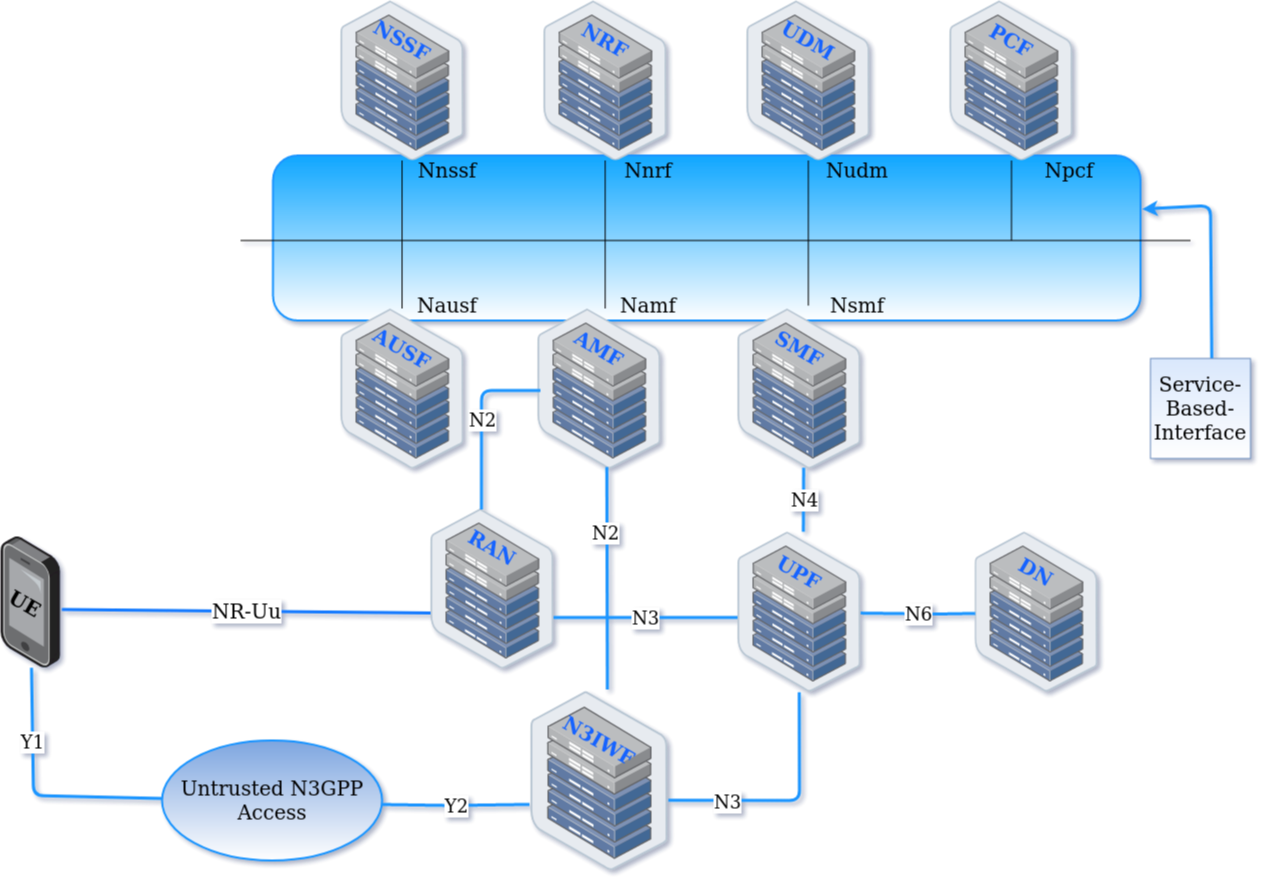
\includegraphics[scale=0.25]{images/Stage2_architecture_of_free5GC.png}
\caption{Stage 2 architecture of free5GC\cite{Free5gc2019}}
\label{fig:Stage2_architecture_of_free5GC}
\end{figure}
    
    
    
\begin{figure}
\centering
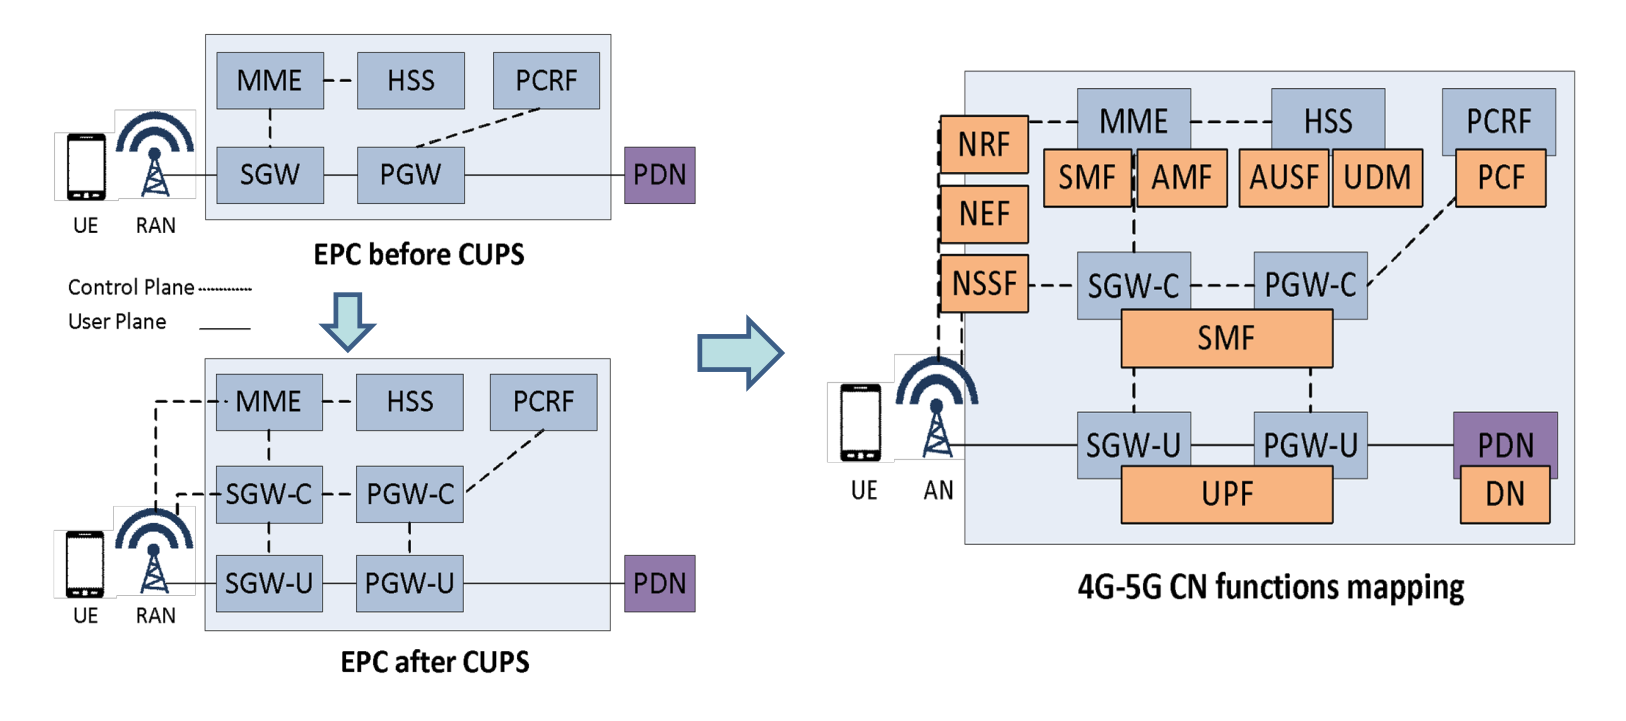
\includegraphics[scale=0.28]{images/oai_epc_core5G1.png}
\caption{5GC Elements corresponding to the 4G \cite{openairinterface2014}}
\label{fig:oai_epc_core5G1}
\end{figure}

    
    
    
    
    
Furthermore, several open source technologies are involved in the study to achieve the aim of this chapter as follows: Docker container, Ansible, Wireshark, Iperf, and dsTest. These terms will be explained in this section and the following sections.


Ansible will make DevOps tasks in this part of the Thesis more effective and less time-consuming. It is an open-source IT automation efficacious tool, which is widely adopted and trusted: because of using simple YAML language and supports different types of infrastructure, e.g., Clouds, Virtual machines. These advantages make it easy for everyone to accept. Furthermore, employ it in all kinds of IT tasks such as configuration management and application deployment. Nevertheless 
, Ansible is agentless or remotely employed.
Besides Ansible components are:
\begin{enumerate}
    \item Ansible Modules: small programs that get executed on target machines.
    \item Ansible Playbook: instructions of the executed programs.
    \item Ansible Inventor: list of hosts where those programs get executed.
\end{enumerate}
Openairinterface (OAI):
The OAI Public License V1.1. Openairinterface permits the researchers, students, and developers to practice and use the OAI 3GPP 5G Core network projects for studying purposes. Figure
\textbf{\ref{fig:oai_epc_core5G1}} depicts the 5GC elements in orange. In other words, it shows fulfilling OAI 5G Core Network components, AMF, SMF, NRF, and UPF (SPGW-U-tiny). Nevertheless, the scenario includes deploying a 5G Service Based Architecture (SBA) core network using docker-compose, dsTest as gNB emulator, attaching and detaching UE, and single public data network (PDN) session establishment.


\begin{figure}
\centering
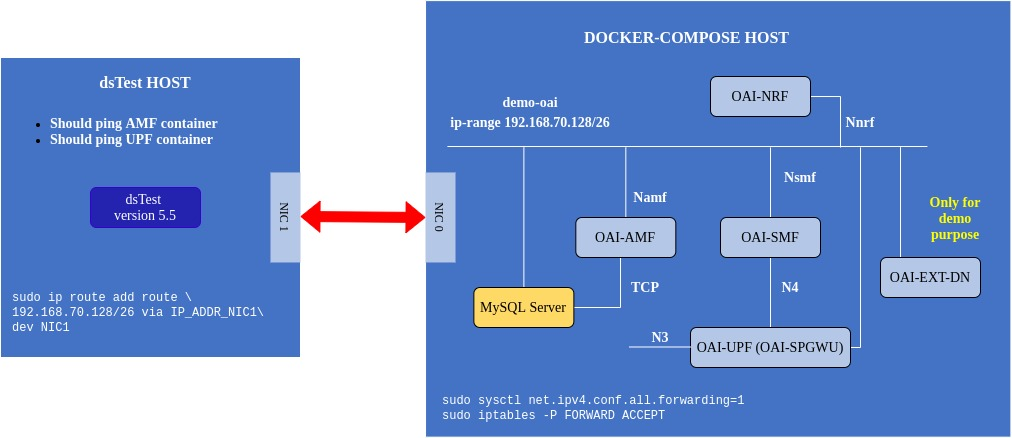
\includegraphics[scale=0.32]{images/OAI5GC_Deployment_using_Docker-Compose_and_Testing_with_dsTest.png}
\caption{5G Core Network Deployment using Docker-Compose and Testing with dsTest \cite{openairinterface2014}}
\label{fig:5GC_Deployment_using_Docker-Compose_and_Testing_with_dsTest}
\end{figure}


The testbed obtains two host machines; As can be noticed in figure
\textbf{\ref{fig:5GC_Deployment_using_Docker-Compose_and_Testing_with_dsTest}}. DsTest host and Docker-compose host, which will be the center of consideration. All 5G core components are running in the Docker-compose host, and they are attached to the same demo-oai. The dstest is deployed in the other machine. The figure shows that the docker-compose host includes an extra container oai-ext-dn, which is only required for the demo goal. Notwithstanding, this container is used in the demo to simulate the downlink traffic. However, because of reasons related to financing, we cannot use a commercial paid gNB emulator (dsTest). Figure \textbf{\ref{fig:5gCN_gnbsim}} shows how can we appropriate gNBsim instead of dstest. Gnbsim is an open-source 5G SA gNB emulator (Rel. 16) for testing 5GS which is written in golang. It simulates NG Application Protocol (NGAP), Non-Access-Stratum (NAS) protocol, and GPRS Tunnelling Protocol User Plane (GTP-U). However, the available gNBsim supports a simulation for one UE and one gNB.




\begin{figure}
\centering
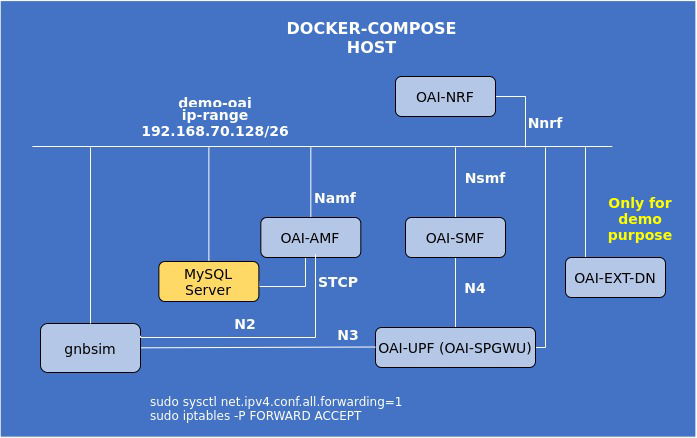
\includegraphics[scale=0.40]{images/5gCN_gnbsim.png}
\caption{5GCN gNBsim  \cite{openairinterface2014}.}
\label{fig:5gCN_gnbsim}
\end{figure}

\clearpage


Pre-requisites of deploying the SA 5GC testbed are described in figure \textbf{\ref{fig:Pre-requisites-oai-cn5g-fed}}. Moreover, the following are the required steps during the setup, which will be explained in detail in the Thesis paper:
\begin{enumerate}
    \item Installation of host operating system Ubuntu 18.04.4 LTS and container operating system Ubuntu 18.04.
    \item Docker engine,  docker-compose, python, and building container images.
    \item Configuring host machines, and configuring OAI 5G Core network functions.
    \item   Deploying OAI 5GC network, getting a gnbsim docker image, and executing gnbsim Scenario.
    \item  Wireshark, and Iperf.
\end{enumerate}
 




\begin{figure}
\centering
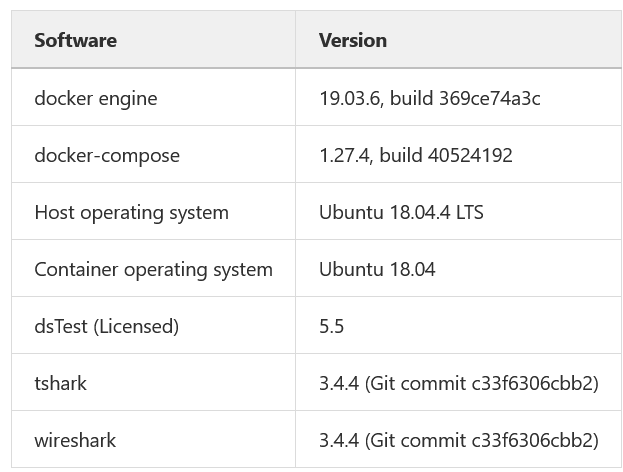
\includegraphics[scale=0.40]{images/Pre-requisites-oai-cn5g-fed.png}
\caption{Pre-requisites OAI 5GCN  \cite{openairinterface2014}.}
\label{fig:Pre-requisites-oai-cn5g-fed}
\end{figure}



 
     
     
   %New colors defined below
\definecolor{codegreen}{rgb}{0,0.6,0}
\definecolor{codegray}{rgb}{0.5,0.5,0.5}
\definecolor{codepurple}{rgb}{0.58,0,0.82}
\definecolor{backcolour}{rgb}{0.95,0.95,0.92}

%Code listing style named "mystyle"
\lstdefinestyle{mystyle}{
  backgroundcolor=\color{backcolour},   commentstyle=\color{codegreen},
  keywordstyle=\color{magenta},
  numberstyle=\tiny\color{codegray},
  stringstyle=\color{codepurple},
  basicstyle=\ttfamily\footnotesize,
  breakatwhitespace=false,         
  breaklines=true,                 
  captionpos=b,                    
  keepspaces=true,                 
  numbers=left,                    
  numbersep=5pt,                  
  showspaces=false,                
  showstringspaces=false,
  showtabs=false,                  
  tabsize=2
}

%"mystyle" code listing set
\lstset{style=mystyle}
  
  
  According to the above, utilizing deployment Docker via Ansible will be more beneficial and operative. Furthermore, the recommendation of Dr.-Ing. Kreuch to present the initially draft instructions of the Ansible playbook of 5GC Network Deployment and Testing with gnbsim will be provided in this section. They are not entirely available yet; because the study and the investigation are ongoing. Nevertheless, this instructions will provide at the abbreviation section in the final thesis paper.  
     
     
     
  Ansible playbook instructions will directly imported and viewed from the files:
  docker-compose.yaml and docker-compose-gnbsim.yaml successively  \cite{openairinterface2014}.
\clearpage


docker-compose.yaml \cite{openairinterface2014}:
%Importing code from file
\lstinputlisting[language=Java, 
caption=docker-compose.yaml\cite{openairinterface2014}.
]{AnsibleFiles/docker-compose.yaml}

\clearpage
Following will be the contents of docker-compose-gnbsim.yaml \cite{openairinterface2014}:

%Importing code from file
\lstinputlisting[language=Java, 
caption=docker-compose-gnbsim.yaml\cite{openairinterface2014}.
]{AnsibleFiles/docker-compose-gnbsim.yaml}

As introduced previously in the draft copy of docker-compose.yaml and docker-compose-gnbsim.yaml both ansible files are preconfigured for executing the gnbsim scenario and will be modified for a test. Then we run the following command to create and launch gnbsim. 
 


%Importing code from file
\lstinputlisting[language=Java, 
caption=Run gnbsim\cite{openairinterface2014}.
]{AnsibleFiles/run_gnbsim.yaml}

Before going to the next step, we need to check that all services' statuses are working fine, as displayed in figure \textbf{\ref{fig:gnbsim_is_healthy}}. 


\begin{figure}
\centering
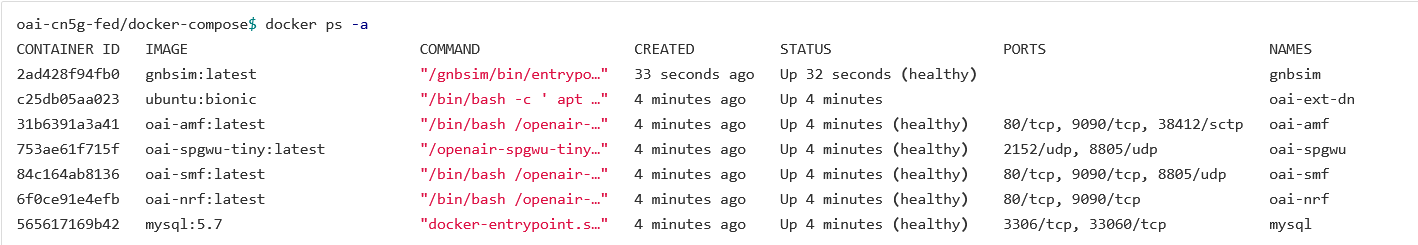
\includegraphics[scale=0.24]{images/gnbsim_is_healthy.png}
\caption{Gnbsim is healthy\cite{openairinterface2014}.}
\label{fig:gnbsim_is_healthy}
\end{figure}
     
     
Momentarily we can implement some traffic tests:
\begin{itemize}
    \item Ping test: Figure \ref{fig:ping_UE_from_external_DN_container} shows us how we ping the UE From the external DN container.
      \item  Iperf test (server/client): 
Between gnbsim UE and the external DN container, we can apply iperf traffic tests because we are able to create any node as an iperf server/client. Figure \ref{fig:iperf_server_traffic_test_between_gnbsim_UE_and_external_DN_node}, figure \ref{fig:iperf_client_traffic_test_between_gnbsim_UE_and_external_DN_node} show the iperf traffic tests and results in the server and client state.
\end{itemize}
   
\begin{figure}
\centering
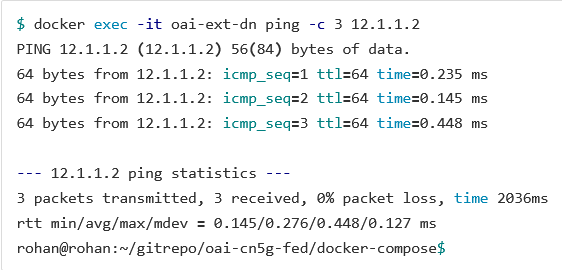
\includegraphics[scale=0.50]{images/ping_UE_from_external_DN_container.png}
\caption{ping UE from external DN container \cite{openairinterface2014}.}
\label{fig:ping_UE_from_external_DN_container}
\end{figure}
 
\begin{figure}
\centering
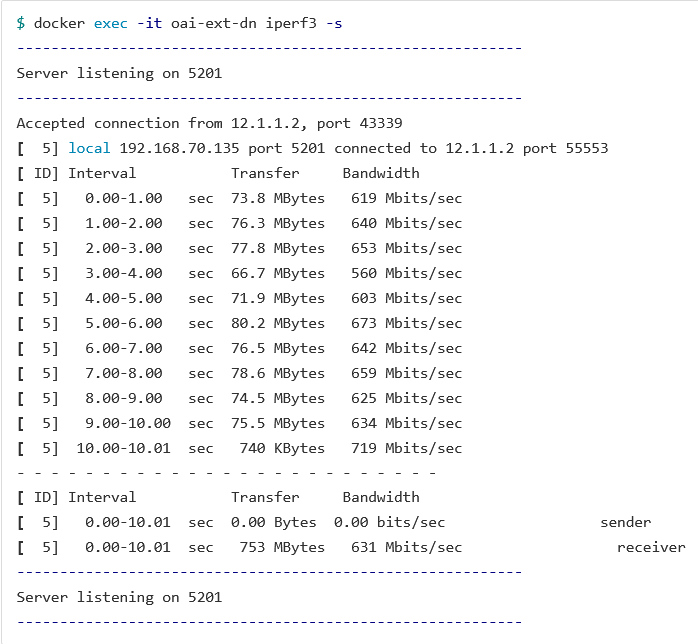
\includegraphics[scale=0.50]{images/iperf_server_traffic_test_between_gnbsim_UE_and_external_DN_node.png}
\caption{Iperf client traffic test between gnbsim UE and external DN node \cite{openairinterface2014}.}
\label{fig:iperf_server_traffic_test_between_gnbsim_UE_and_external_DN_node}
\end{figure}

\begin{figure}
\centering
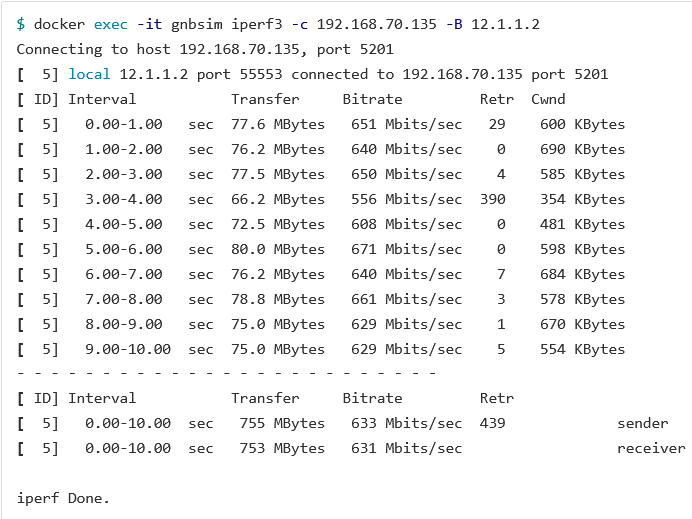
\includegraphics[scale=0.50]{images/iperf_client_traffic_test_between_gnbsim_UE_and_external_DN_node.png}
\caption{Iperf client traffic test between gnbsim UE and external DN node \cite{openairinterface2014}.}
\label{fig:iperf_client_traffic_test_between_gnbsim_UE_and_external_DN_node}
\end{figure}

    %\section{Evaluation: Scalability of the Current Implementation}\label{sec:evaluation}
\section{\textbf{Evaluation }}\label{sec:evaluation} 


Wireshark and Iperf, as open-source tools, are employed to take measurements and read the values to get the best tolerable results. 
Wireshark is a free open-source network packet analyzer. It is used to capture data packets and display the most accurate details achievable about them. Similarly, Iperf is an open-source tool for active measurements of the peak possible bandwidth on IP networks. Besides, it supports harmonizing many factors related to timing and protocols ( Transmission Control Protocol (TCP), User Datagram Protocol (UDP), Stream Control Transmission Protocol (SCTP) with IPv4 and IPv6)\cite{iperf2021}.
Other significant advantages are that Iperf can be utilized in two forms: server and client modes. In addition, it supports End-to-end (E2E) testing and affords a throughput measurement report between the two ends in one or both directions. It handles both data streams: Transmission Control Protocol (TCP) or User Datagram Protocol (UDP). The primary target of (E2E) testing is to examine the end user's activity by simulating the real user scenario and validating the system under test and its elements for combination and data integrity. It is beneficial for analyzing network traffic in real-time.
Figure \textbf{\ref{fig:5gcn-deployment-gnbsim}} presents the Wireshark user interface. We start the 5GC Network components: NRF, Mysql, AMF, SMF, and SPGWU. Then we capture packets on the docker-compose host as shown in the bottom section. The initial data exchanges between the core network components are evident here.
Furthermore, capturing these packets is fundamental, allowing us to see the expected exchange between SMF, RNF, and UPF. SMF can discover UPF using the service discovery feature of NRF. The core network should be correctly configured and healthy, as displayed in figure
\textbf{\ref{fig:corenetwork_are_healthy}}. The completely evaluation process, including taking measurements and monitoring time synchronization, reliability, latency, and determinism, will be explained in detail in the master's paper\cite{openairinterface2014}.
 
 


\begin{figure}
\centering
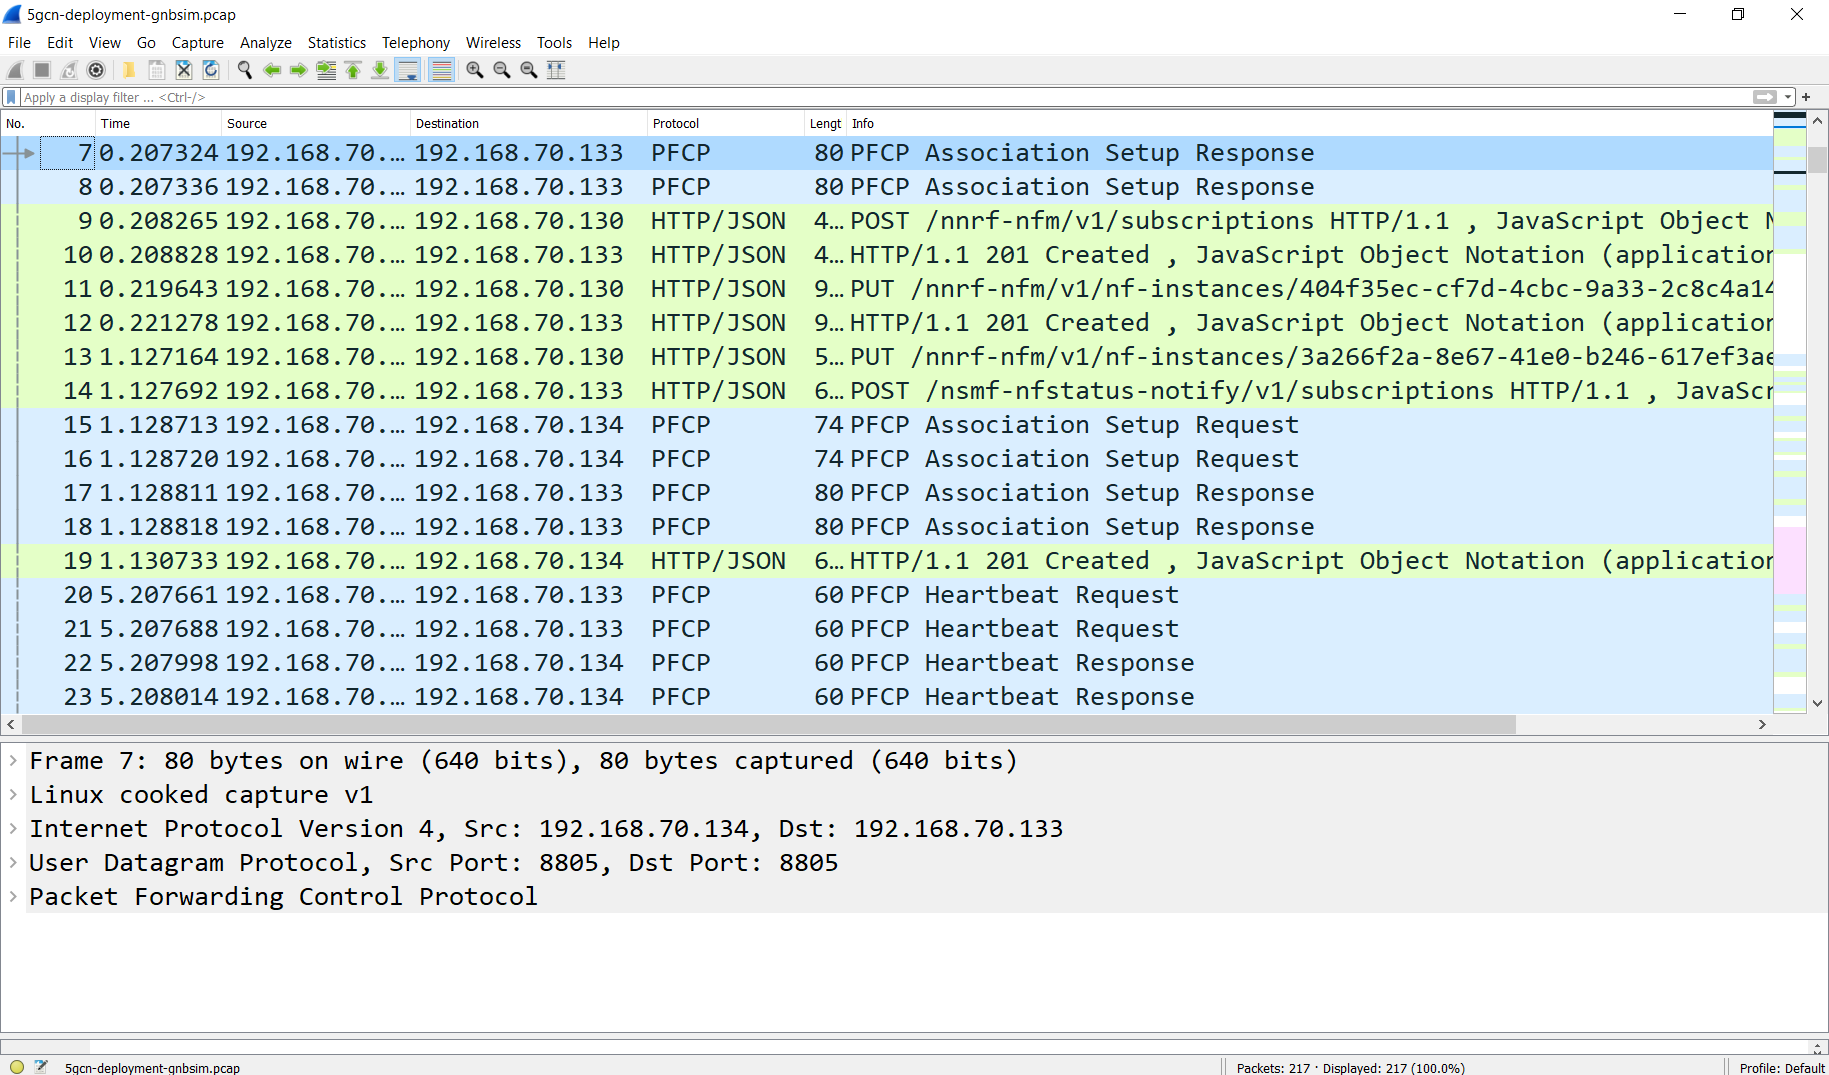
\includegraphics[scale=0.18]{images/5gcn-deployment-gnbsim.png}
\caption{5GC Network Deployment gNBsim \cite{openairinterface2014}}
\label{fig:5gcn-deployment-gnbsim}
\end{figure}






\begin{figure}
\centering
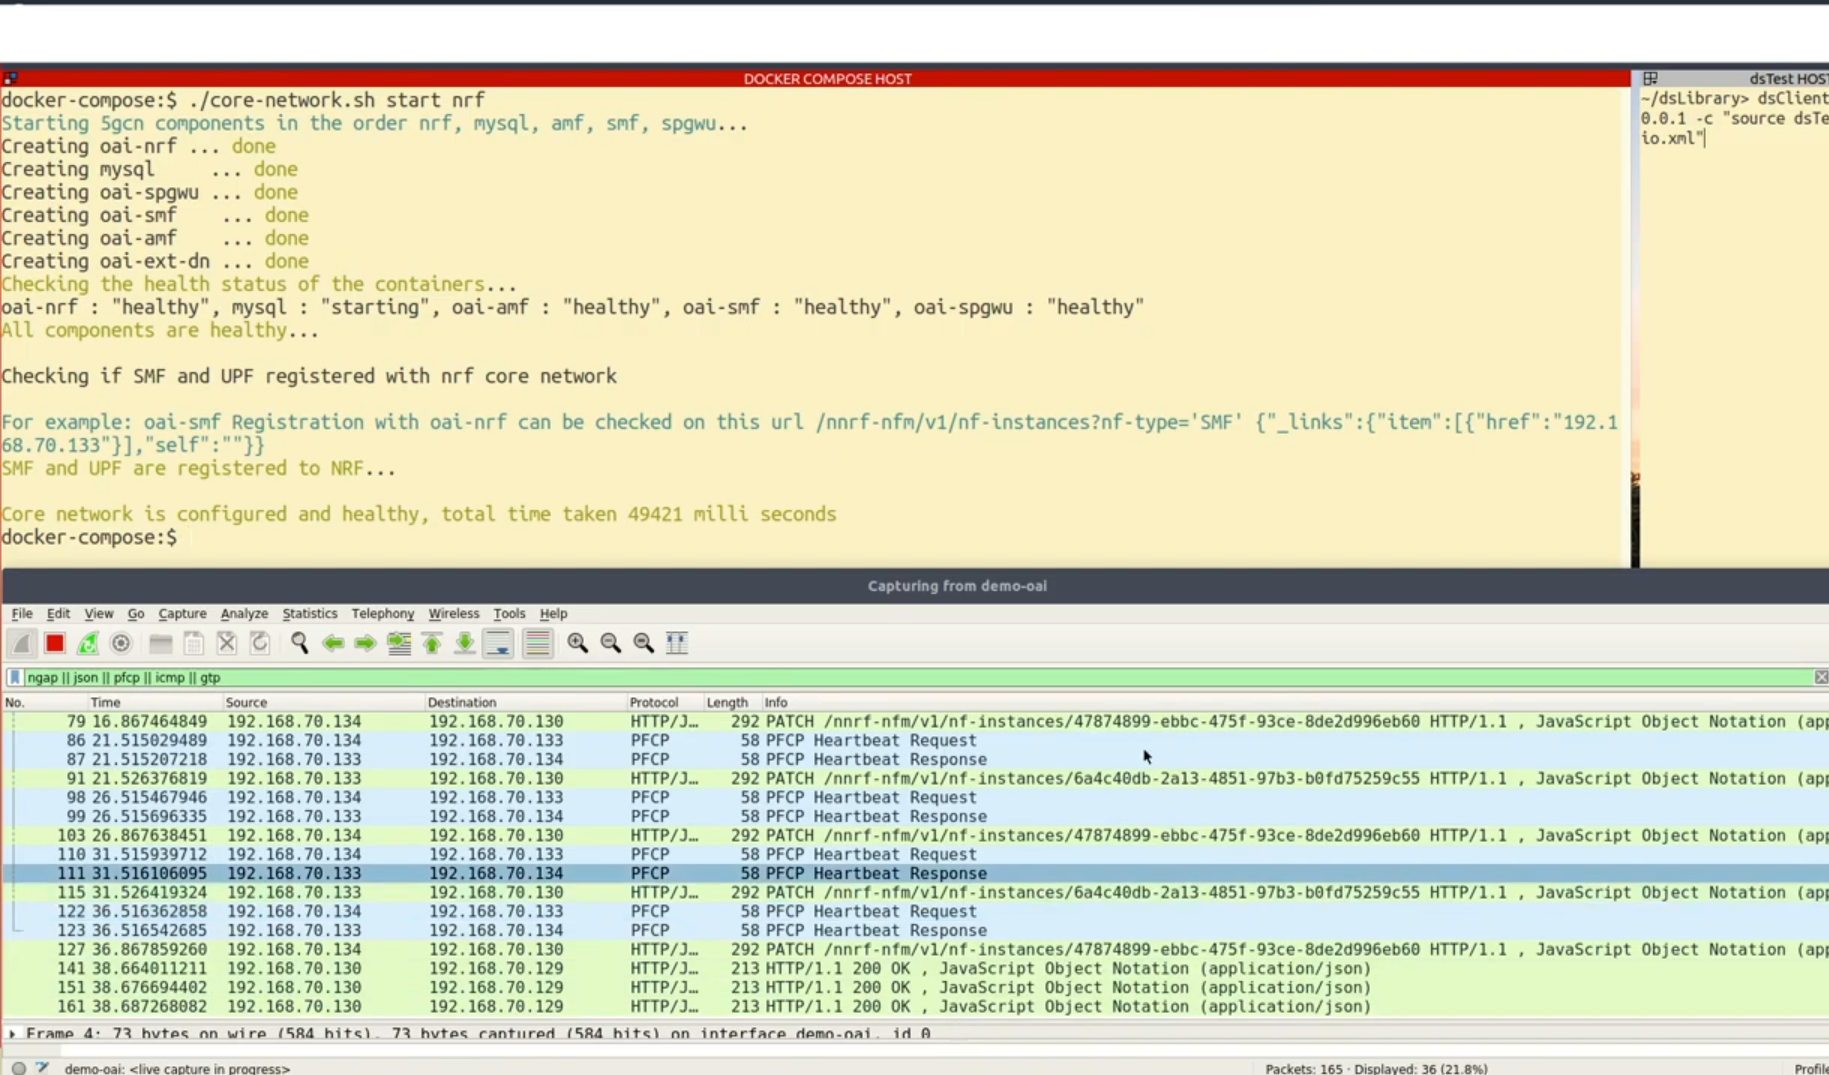
\includegraphics[scale=0.18]{images/corenetwork_are_healthy.png}
\caption{Core Network are healthy and configured \cite{openairinterface2014}.}
\label{fig:corenetwork_are_healthy}
\end{figure}


 

%mmm\subsection{Comparative analysis of Open Source 5G Core implementations (NextEPC, Free5GC, ...) } 
 


% MMM \subsection{Use cases of this Architecture}\label{Use cases of this Architecture}


%-------------------------------------------------------------------------------
%Evaluation: How does it really work in practice? Provide real or simulated
%performance metrics, end-user studies, mention external technology adoptors,
%if any, etc.

%This section presents the detailed results you have obtained. If the paper
%is theoretical, you might want to show curves obtained from your equations.
%If the paper is experimental, you will be presenting curves showing the
%measurement results. In order to choose the proper curves to present, you
%must first be clear what point you are trying to convey to the reader. The 
%curves can then be chosen to illustrate this point. Whether your paper is
%theoretical or experimental, you must provide a careful interpretation of
%what your results mean and why they behave as they do.
%-------------------------------------------------------------------------------
% This section presents the detailed results obtained. It contains the results
% obtained from the analytical model, the emulations and the simulations realized
% as well as the interpretation and discussion of them. 
%-------------------------------------------------------------------------------
% The goals of the study,
% The system boundaries
% System services and possible outcomes
% Selected performance metrics
% System and workload parameters
% Factors and their values
% Evaluation techniques
% Selected workload
% Design of the experiments
% Analysis and interpretation of the data
% Presentation of the results
%------------------------------------------------------------------------------_

%mmm Evaluation: How does it really work in practice? Provide real or simulated performance metrics, end-user studies, mention external technology adopters, if any, and so on.                                %This section presents the detailed results you have obtained. If the paper is theoretical, you might want to show curves obtained from your equations. 
%If the paper is experimental, you will be presenting curves showing the  measurement results. In order to choose the proper curves to present, you must first be clear what point you are trying to convey to the reader. The curves can then be chosen to illustrate this point. Whether your paper is theoretical or experimental, you must provide a careful interpretation of what your results mean and why they behave as they do.

\section{\textbf{Expected Result}}\label{Expected Result}
%\subsection{Study of what is needed}\label{Study of what is needed}
%\subsection{Best effort testbed environment}\label{Best effort testbed environment}


The expected result usually will be:  releasing a signal with 5g logo and uplink or downlink data after turning on the WiFi in all connected mobile phones, the ability to connect a massive number of mobile phones, all phones can watch HD video at the same time. However, the expected result will be limited to the captured packets in Wireshark and Iperf tools because of international health status and costs.
As we previously explained, The initial data exchanges between the core network components are evident At the bottom window of the Wireshark. Additionally, capturing these packets is significant, seeing the expected exchange between SMF, RNF, and UPF. Furthermore, SMF can discover UPF using the service discovery feature of NRF. We can observe intermediary request responses between UPF and SMF. Wireshark shows the signaling process and when UE is accessed, such as registration, authentication, PDU session establishment, an uplink, or downlink GTP packet. Within viewing the AMF log, which showed in figure  \ref{fig:amf_log_user_observed}, we can see that there is already a user Observed.
 

 


\begin{figure}
\centering
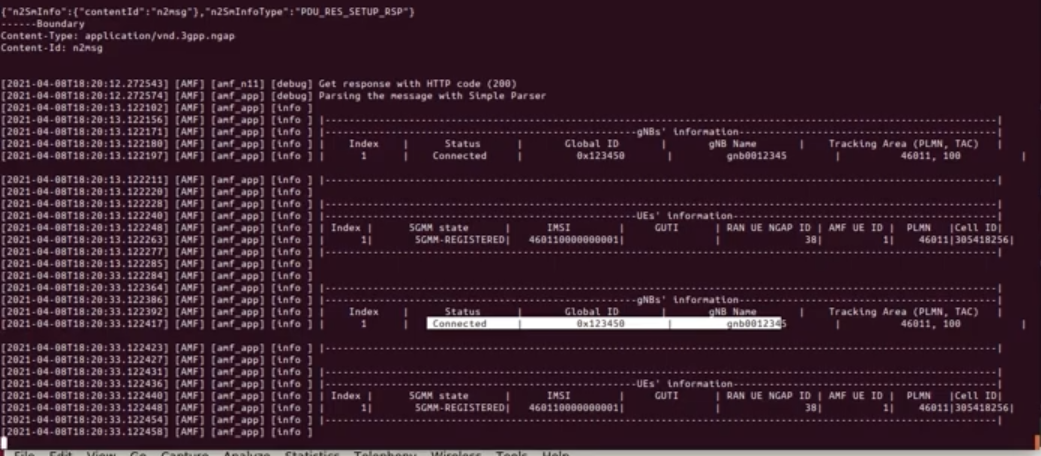
\includegraphics[scale=0.33]{images/amf_log_user_observed.png}
\caption{A user observed in AMF log \cite{openairinterface2014}.}
\label{fig:amf_log_user_observed}
\end{figure}

 
In the SMF log, we can understand that the IP sent by SMF is the same as the phone. 
Nevertheless, it displays data and other session messages. After stopping the 5GC components services, we can see that the phone loses the signal in case of the possibility to use a phone. All the logs file, including 5gcn-deployment-gnbsim.pcap, amf.log, initialmessage.log, smf.log, nrf.log, and spgwu.log will be viewed in the final paper.
   
 
    \section{\textbf{Work Plan}}\label{sec:conclusions}


%-------------------------------------------------------------------------------
%In general a short summarizing paragraph will do, and under no circumstances
%should the paragraph simply repeat material from the Abstract or Introduction.
%In some cases it's possible to now make the original claims more concrete,
%e.g., by referring to quantitative performance results.

%The further work material is important -- part of the value of a paper is
%showing how the work sets new research directions. (1) If you're actively
%engaged in follow-up work, say so. E.g.: "We are currently extending the
%algorithm to... blah blah, and preliminary results are encouraging." This
%statement serves to mark your territory. (2) Conversely, be aware that some
%researchers look to Future Work sections for research topics. 

%This section should summarize what has  been accomplished in the paper. Many
%readers will read only the Introduction and Conclusion of your paper. The
%Conclusion should be written so they can be understood by someone who has not
%read the main work of the paper.

%-------------------------------------------------------------------------------
%We have shown that\dots. The crucial results are\dots.  
%-------------------------------------------------------------------------------
 
The 5G-TSN integration is a crucial topic of importance for all communication companies.The 5G and TSN mixture is ideal for intelligent factories, given ultra-reliability and low latency characteristics. Although, a particular level of integration of the couple technologies is required to present End-to-End Ethernet connectivity to match the industrial requirements. That allows us to imagine; How much the integrated time synchronization through wired TSN and wireless 5G domains affords a regular reference time for industrial endpoints. 5G is also integrated with the given TSN tool used in an unusual deployment to accommodate limited low latency. End-to-End Ultra-reliability and high availability are granted by the arrangement of the disjoint forwarding paths of the 5G and TSN segments \cite{Ericsson2019}. This study aims to understand the open-source 5G core Network benefits and Time-sensitive Network (TSN) features. The integration between both technologies is the key To achieve eMBB,  mMTC, and uRLLC. In this Thesis, we tried to design and implement the best effort testbed environment that can be provided by integrating open source 5GC and TSN. Chapter 2 (State of the Art) in the thesis paper can give us all the background that we need to understand this thesis. It provides more knowledge about architecture. In addition to that, we will also deploy a Standalone 5GC Network.
Chapters 4, 5, and 6 (Design and Specifications) explain the implementation's needed knowledge in detail.
Last but not least, Wireshark and Iperf are utilized to achieve a Comparative Analysis of OS 5G Core Implementations and Design and Evaluation of a 5G Testbed.



%\sidenote{results}
%\todomid{We have shown that\dots}.
%\todomid{The crucial results are\dots.}

%-------------------------------------------------------------------------------
%Recipient of the results/improvements. Who gaines provit from this?
%-------------------------------------------------------------------------------
%\sidenote{benefits}
%\todomid{The presented work provides %potential benefits for\ldots}

%-------------------------------------------------------------------------------
%Further work: start with short-term, then long-term ojectives.
% -------------------------------------------------------------------------------



%\subsection{Enhancement of hardware-supported scheduled TSN traffic (out of scope of this thesis)}\label{Enhancement of hardware-supported scheduled TSN traffic (out of scope of this thesis)}
%\subsection{Integration of hardware-supported scheduled TSN traffic (out of scope of this thesis)}\label{Integration of hardware-supported scheduled TSN traffic (out of scope of this thesis)}

%\subsection{Summary}\label{Summary}
%\subsection{Conclusion and Future Work}\label{Conclusion and Future Work}


\subsection{\textbf{Thesis Structure}}\label{Structure of the Thesis} 



 
\begin{figure}
Thesis Structures illustrated in figures \textbf{\ref{fig:Thesis-TOC1}},\textbf{\ref{fig:Thesis-TOC2}},\textbf{\ref{fig:Thesis-TOC3}},\textbf{\ref{fig:Thesis-TOC4}},


 \end{figure}
\begin{figure}
 
\centering
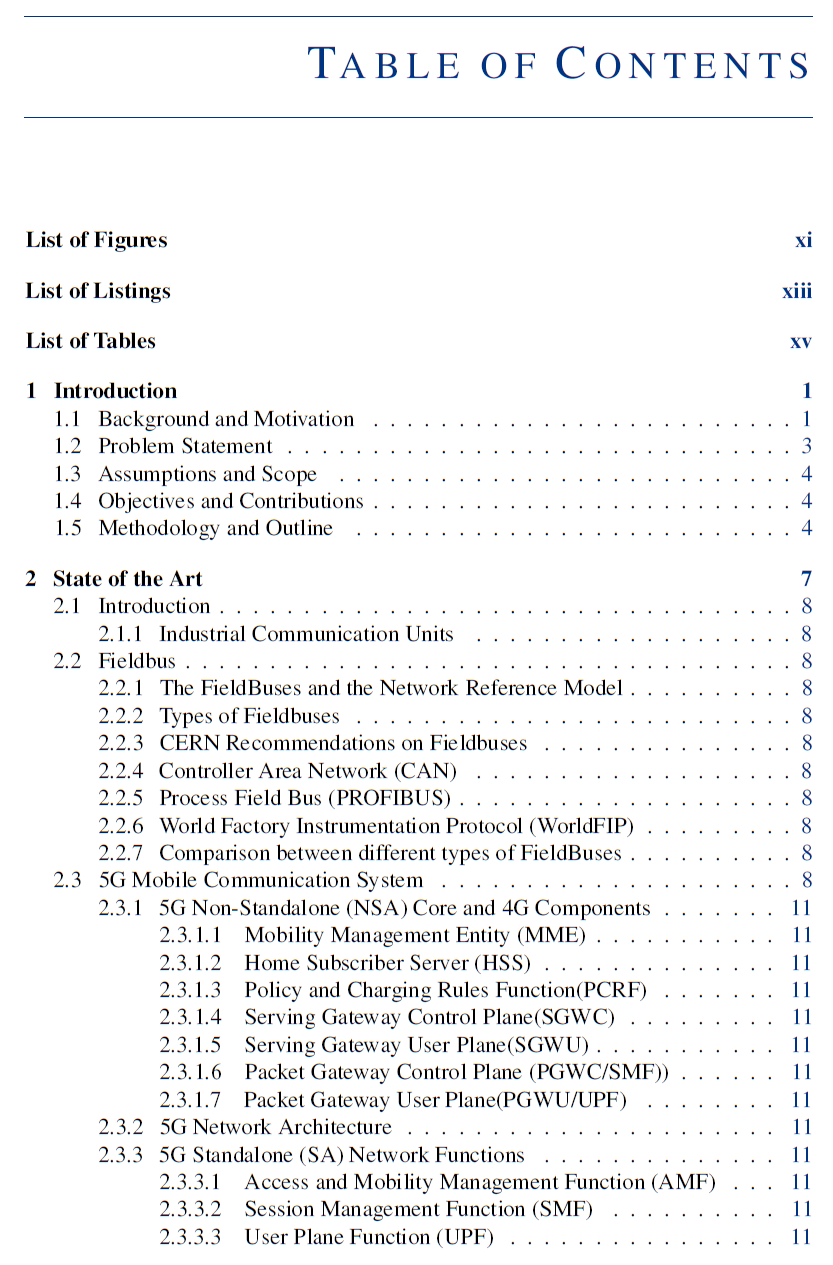
\includegraphics[scale=0.41]{images/Thesis-TOC1.png} 
\caption{Thesis Structure TOC1}
\label{fig:Thesis-TOC1}
 

 \end{figure}
\begin{figure}

 
  \centering
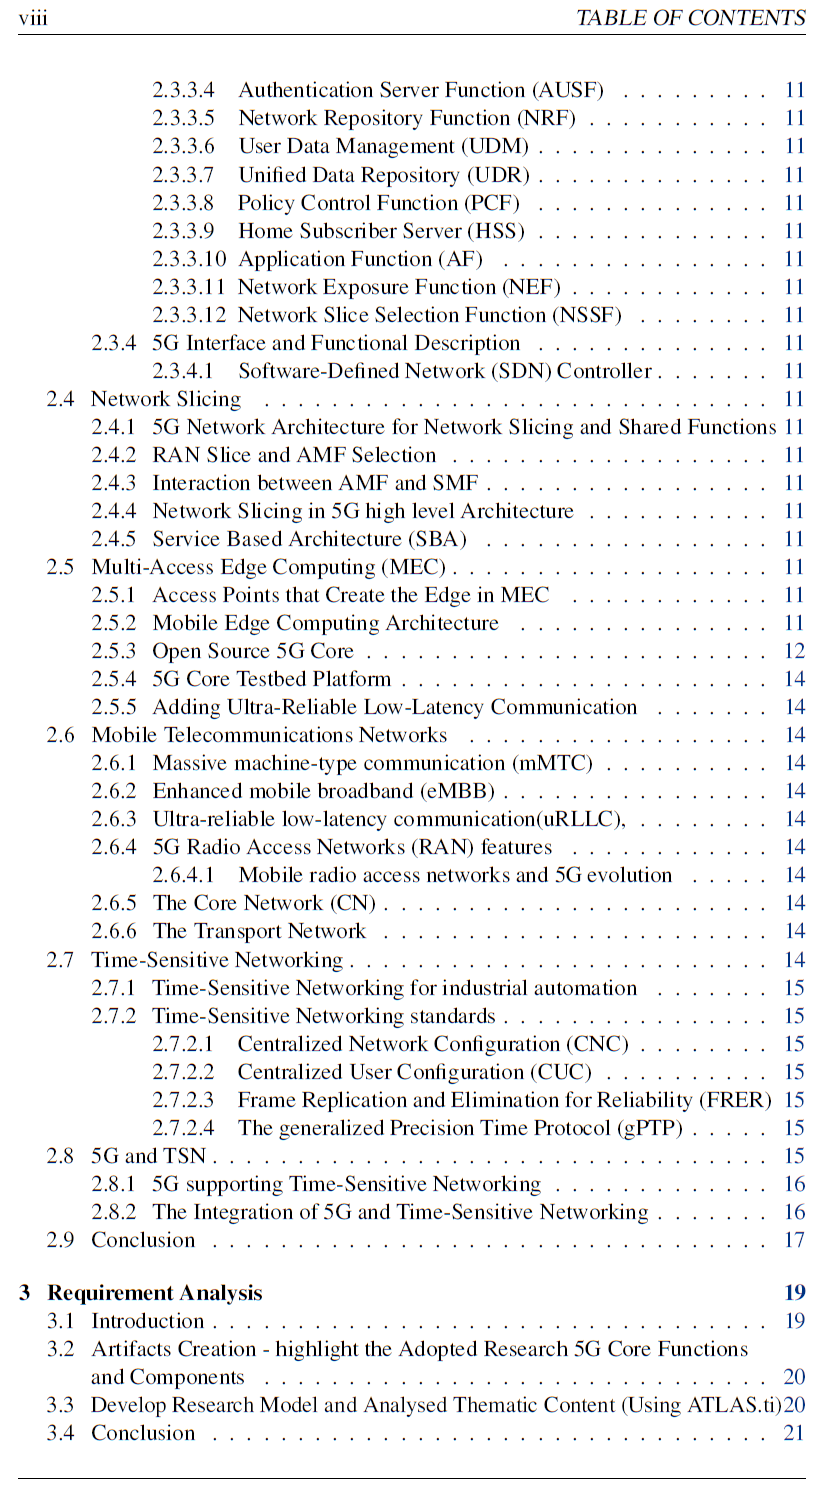
\includegraphics[scale=0.39]{images/Thesis-TOC2.png} 
\caption{Thesis Structure TOC2}
\label{fig:Thesis-TOC2}
 \end{figure}
 
 
 
\begin{figure}
\centering
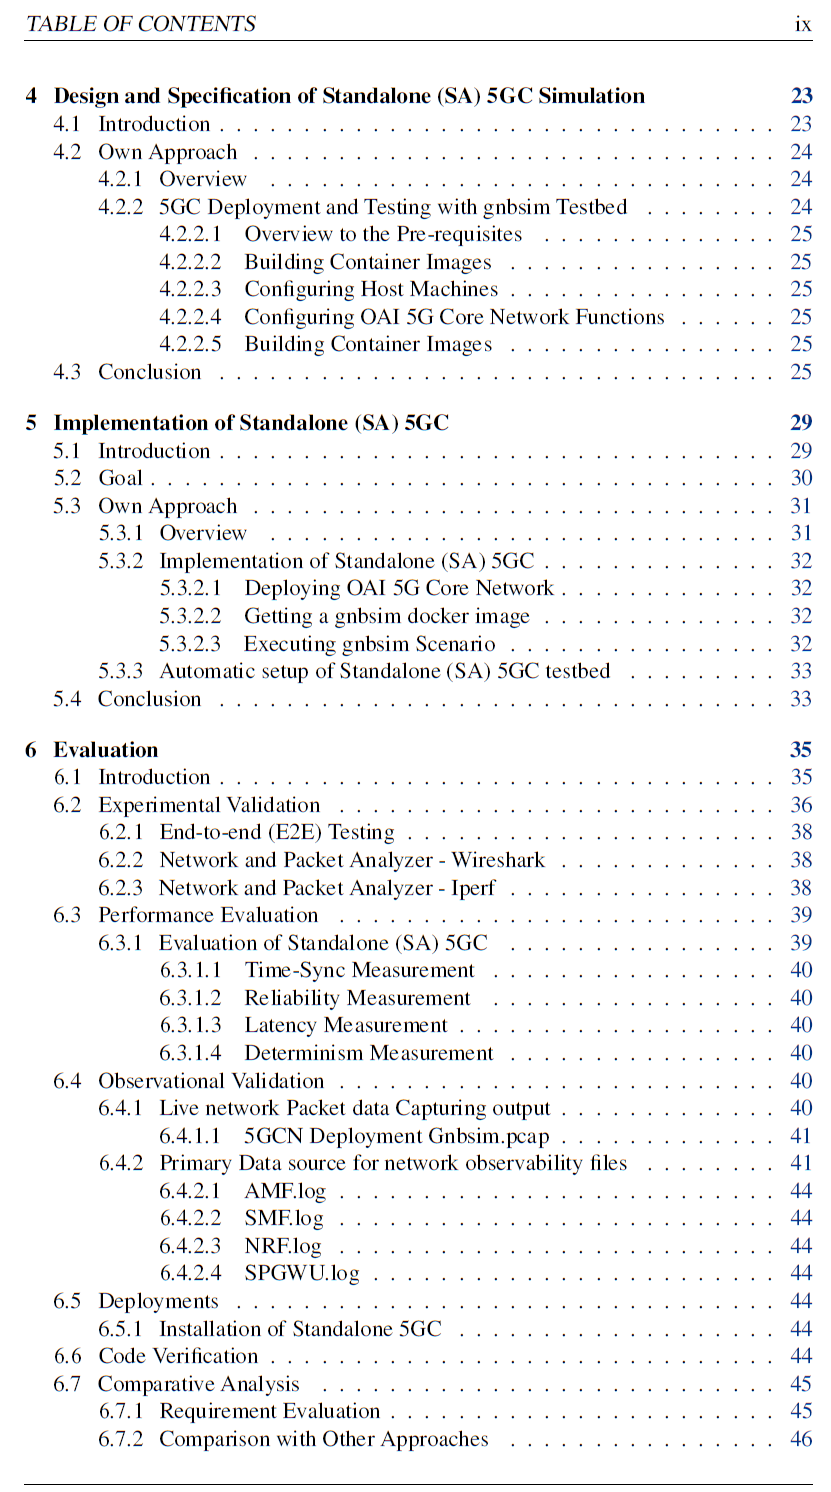
\includegraphics[scale=0.41]{images/Thesis-TOC3.png} 
\caption{Thesis Structure TOC3}
\label{fig:Thesis-TOC3}
 \end{figure}
 
\begin{figure}
\centering
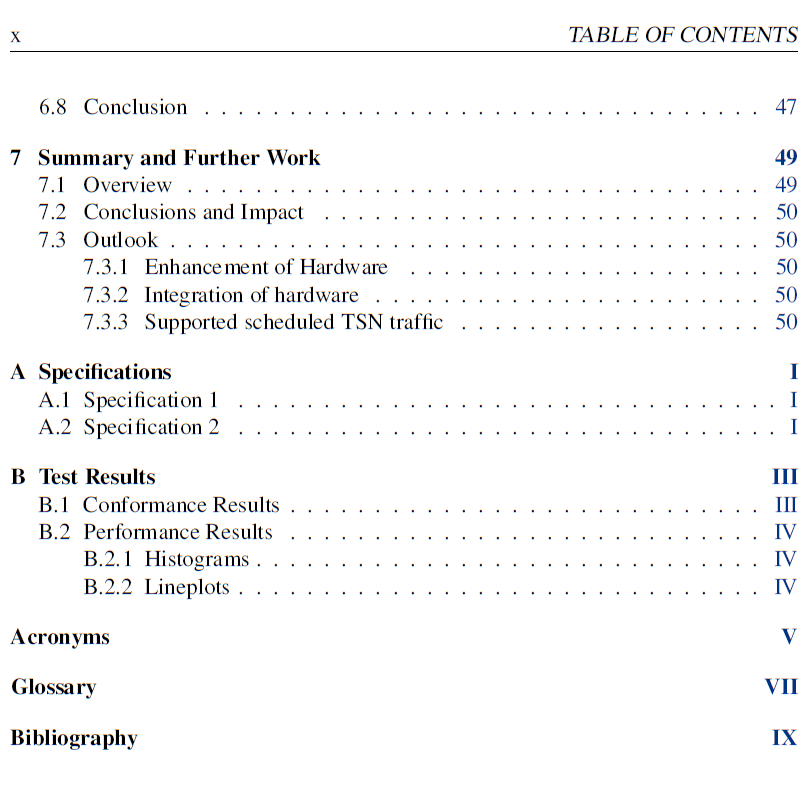
\includegraphics[scale=0.40]{images/Thesis-TOC4.png}
\caption{Thesis Structure TOC4}
\label{fig:Thesis-TOC4}
 \end{figure}
 
\clearpage


\subsection{\textbf{Gantt}}\label{Gantt timeline- with milestones and overall planned duration}

As mandate by Regulations Governing General Study and Examination Procedures (AllgStuPO), the period to work for a master thesis should be in six months.
The proposed timeline to commence this work is depicted in figure \textbf{\ref{fig:Thesis_High-level_Timeline}}
below.
 
 
 
\begin{figure}
 
\centering
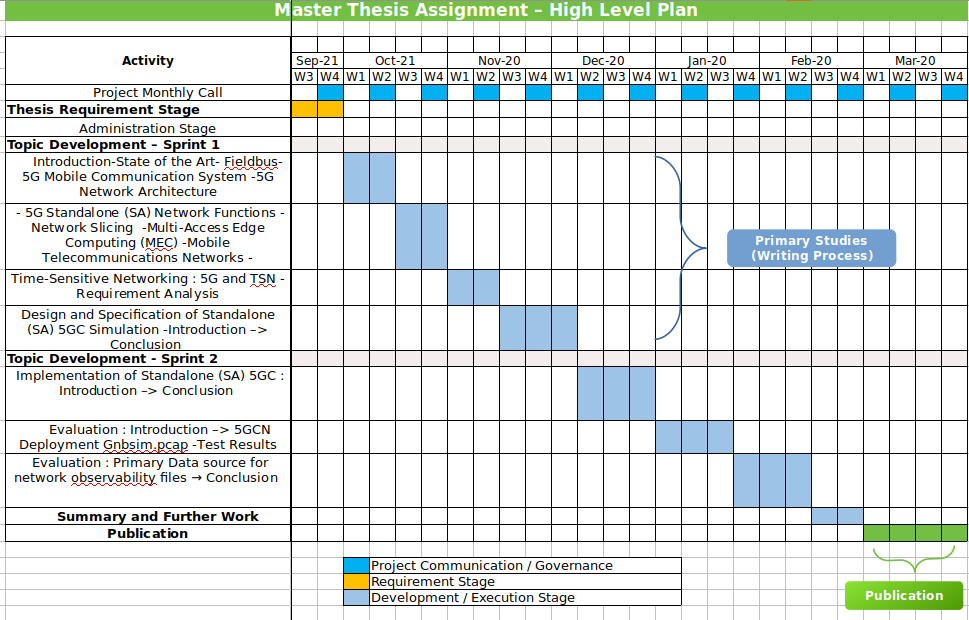
\includegraphics[scale=0.35]{images/Timeline_OS_5GC.png}
\caption{Master Thesis High level Timeline.}
\label{fig:Thesis_High-level_Timeline}
  \end{figure}

 
%\sidenote{gap 2}
%\todotext{related work 2}

%\sidenote{gap 3}
%\todotext{related work 3}

%\sidenote{issue}
%\todotext{outstanding problem}


    %\section{Acknowledgments}\label{sec:ack}
%\metaThanks%

    

    
    
    
   
    
    %\bibliographystyle{IEEEtran} % enable for bibtex
    % enable for bibtex
    \printbibliography% enable for biber style
    % to show unreferenced publications ------------------------------------- */
    %\bibliographystyle{unsrt}
    %\cite{dummy}
    %\nocite{*}
    %------------------------------------------------------------------------ */

    % /* -------------------------------------------------------------------- */
    %\backmatter
\end{document}
% /* ------------------------------------------------------------------------ */
